%Version 3.1 December 2024
% Springer Nature journal article template (sn-jnl), see sn-article.tex and user-manual.pdf
% in the template package. Compile with pdfLaTeX + BibTeX:
%   pdflatex main && bibtex main && pdflatex main && pdflatex main
%
%%\documentclass[referee,pdflatex,sn-mathphys-num]{sn-jnl}% double line spacing for peer review
%%\documentclass[lineno,pdflatex,sn-mathphys-num]{sn-jnl}% line numbers in the margin
\documentclass[pdflatex,sn-mathphys-num]{sn-jnl}% Math and Physical Sciences Numbered Reference Style

%%%% Standard Packages
\usepackage{graphicx}%
\usepackage{multirow}%
\usepackage{amsmath,amssymb,amsfonts}%
\usepackage{amsthm}%
\usepackage{mathrsfs}%
\usepackage[title]{appendix}%
\usepackage{xcolor}%
\usepackage{textcomp}%
\usepackage{manyfoot}%
\usepackage{booktabs}%
\usepackage{algorithm}%
\usepackage{algorithmicx}%
\usepackage{algpseudocode}%
\usepackage{listings}%
%%%% Additional packages
\usepackage{array}%
\usepackage{tabularx}%
%%%%

\newcolumntype{L}{>{\raggedright\arraybackslash}X}

%% Unnumbered, titled text blocks for the worked examples and the plain-language box,
%% set with the template's definition style (bold head, roman text).
\theoremstyle{thmstylethree}%
\newcommand{\textblockname}{}%
\newtheorem*{textblock*}{\textblockname}%
\newenvironment{workedexample}[1]{\renewcommand{\textblockname}{Worked example #1}\begin{textblock*}}{\end{textblock*}}%
\newenvironment{plainwords}{\renewcommand{\textblockname}{In simple words}\begin{textblock*}}{\end{textblock*}}%

\raggedbottom

\begin{document}

\title[Energy-Efficient Priority Scheduling for Task Allocation in 6G Edge Computing]{Energy-Efficient Priority Scheduling for Task Allocation in 6G Edge Computing}
\subtitle{Deadline-aware queues and guarded CPU slow-down on top of the EdgePlus scheduler}

%% To mark the corresponding author, use \author*[1]{...}\email{...}
\author[1]{\fnm{Keerat} \sur{Malhotra}}

\author[1]{\fnm{Bhavya} \sur{Maheshwari}}

\author[1]{\fnm{Bhumika} \sur{Aswal}}

\affil[1]{\orgname{Netaji Subhas University of Technology}, \orgaddress{\city{New Delhi}, \country{India}}}

\abstract{Edge computing places small servers close to the devices that use them, so that results come back
quickly. In a 6G smart city these servers receive a constant stream of tasks from sensors, and the tasks have
very different deadlines: an air-pollution alert may need an answer within seconds, while a logging job can wait
ten minutes. EdgePlus, a recent scheduler published in the \emph{IEEE Internet of Things Journal}, uses
reinforcement learning to decide which server each task should go to. Once a task reaches a server, however,
EdgePlus treats all tasks alike: they wait in arrival order and run at full CPU speed.

We add two simple rules inside every server. The first is a form of priority scheduling: the server always runs
the waiting task whose deadline is closest, and it drops a task as soon as that task can no longer finish in
time. The second saves energy: when nothing else is waiting, the server lowers its CPU speed for a task that has
time to spare, but never by more than 1.5 seconds of extra running time. We rebuilt EdgePlus in a simulator,
trained it, and tested the same trained model with and without our rules on two datasets: the CityPulse data
used by EdgePlus, and real sensor data collected on public buses in Delhi (AirDelhi).

At the heaviest load we tested (150{,}000 tasks in ten minutes), the share of tasks finished on time rises from
80.5\% to 99.7\% on CityPulse and from 73.0\% to 96.5\% on AirDelhi, and missed urgent tasks fall from 55.4\% to
0.07\% on CityPulse. At light load, energy per task falls by 19.8\% while every task still finishes on time. The
price is that relaxed tasks wait longer: the overall 95th-percentile latency at heavy load rises from 148\,s to
298\,s on CityPulse, although those tasks still meet their own deadlines. The paper explains each idea from first
principles, with worked examples, so that readers who are new to the field can follow it.}

\keywords{6G, edge computing, task allocation, priority scheduling, earliest deadline first, energy efficiency, DVFS, reinforcement learning}

\maketitle

%=====================================================================================================
\section{Introduction}
%=====================================================================================================

Picture a city with thousands of air-quality sensors on lamp posts, rooftops and buses. Every few seconds each
sensor sends a reading, and every reading needs a little computing: checking whether pollution has crossed a
dangerous level, updating a pollution map, or simply storing the value for later. Some of these jobs are urgent.
If fine dust suddenly spikes next to a school, an alert that arrives a minute late is of little use. Other jobs
are relaxed: a reading that is only being logged can wait ten minutes and nobody will notice.

Sending all of this work to a big cloud data centre far away adds delay. \emph{Edge computing} solves part of the
problem by placing smaller servers close to the sensors, for example next to the mobile base stations of a
city, so that answers come back faster. Sixth-generation (6G) mobile networks, expected around 2030, are being
designed to connect very large numbers of such devices with very low delay. Edge servers are still limited,
though. When many tasks arrive at once, some of them have to wait, and some miss their deadlines.

A recent and strong answer to the question \emph{``which server should each task go to?''} is EdgePlus
\cite{edgeplus2026}, published in the \emph{IEEE Internet of Things Journal} in 2026. EdgePlus uses
reinforcement learning: a program that learns, by trial and error in a simulated city, how to pick a good
server for each task. Before it chooses, EdgePlus removes every server that clearly cannot finish the task in
time. The paper reports that this ``feasibility-first'' design meets more deadlines under heavy load than four
other learning-based schedulers.

What EdgePlus does not change is what happens \emph{after} the choice. Once a task reaches a server, EdgePlus
assumes that it waits in line in arrival order (\emph{first come, first served}) and that the server always runs
at full CPU speed. When we rebuilt EdgePlus, we noticed two consequences:
\begin{enumerate}
\item \textbf{Urgent tasks wait behind relaxed ones.} At the heaviest load (150{,}000 tasks arriving in ten
minutes), 55\% of the urgent tasks missed their deadline, while only 0.03\% of the relaxed logging tasks did.
The servers had enough capacity overall; they were simply working on the wrong tasks first.
\item \textbf{Spare time is wasted as energy.} At light load almost every task finishes long before its deadline.
A CPU that runs a little slower uses noticeably less energy, so finishing early at full speed wastes energy for
no benefit.
\end{enumerate}

This paper adds two simple rules inside every server to fix these two problems:
\begin{itemize}
\item \textbf{Rule 1, priority scheduling by deadline.} The server always runs the waiting task whose deadline is
closest. This is called \emph{earliest deadline first} (EDF). If a task can no longer finish in time even at full
speed, the server drops it instead of letting it block everyone else.
\item \textbf{Rule 2, energy saving.} When nothing else is waiting, the server may lower its CPU speed for a task
that has time to spare. The slow-down may use at most 80\% of the spare time and may add at most 1.5 seconds.
Lowering the speed of a processor in this way is called \emph{dynamic voltage and frequency scaling} (DVFS); we
call our careful version \emph{guarded DVFS}.
\end{itemize}

Both rules are fixed rules, not learned ones. This means they can be switched on for an EdgePlus model that has
already been trained, with no extra training. It also makes the comparison very clean: in every experiment
below, the trained EdgePlus model is exactly the same, and only the server rules change.

Figure~\ref{fig:overview} shows where everything sits. The blue parts belong to EdgePlus; the orange parts are
what we add.

\begin{figure}[!htbp]
\centering
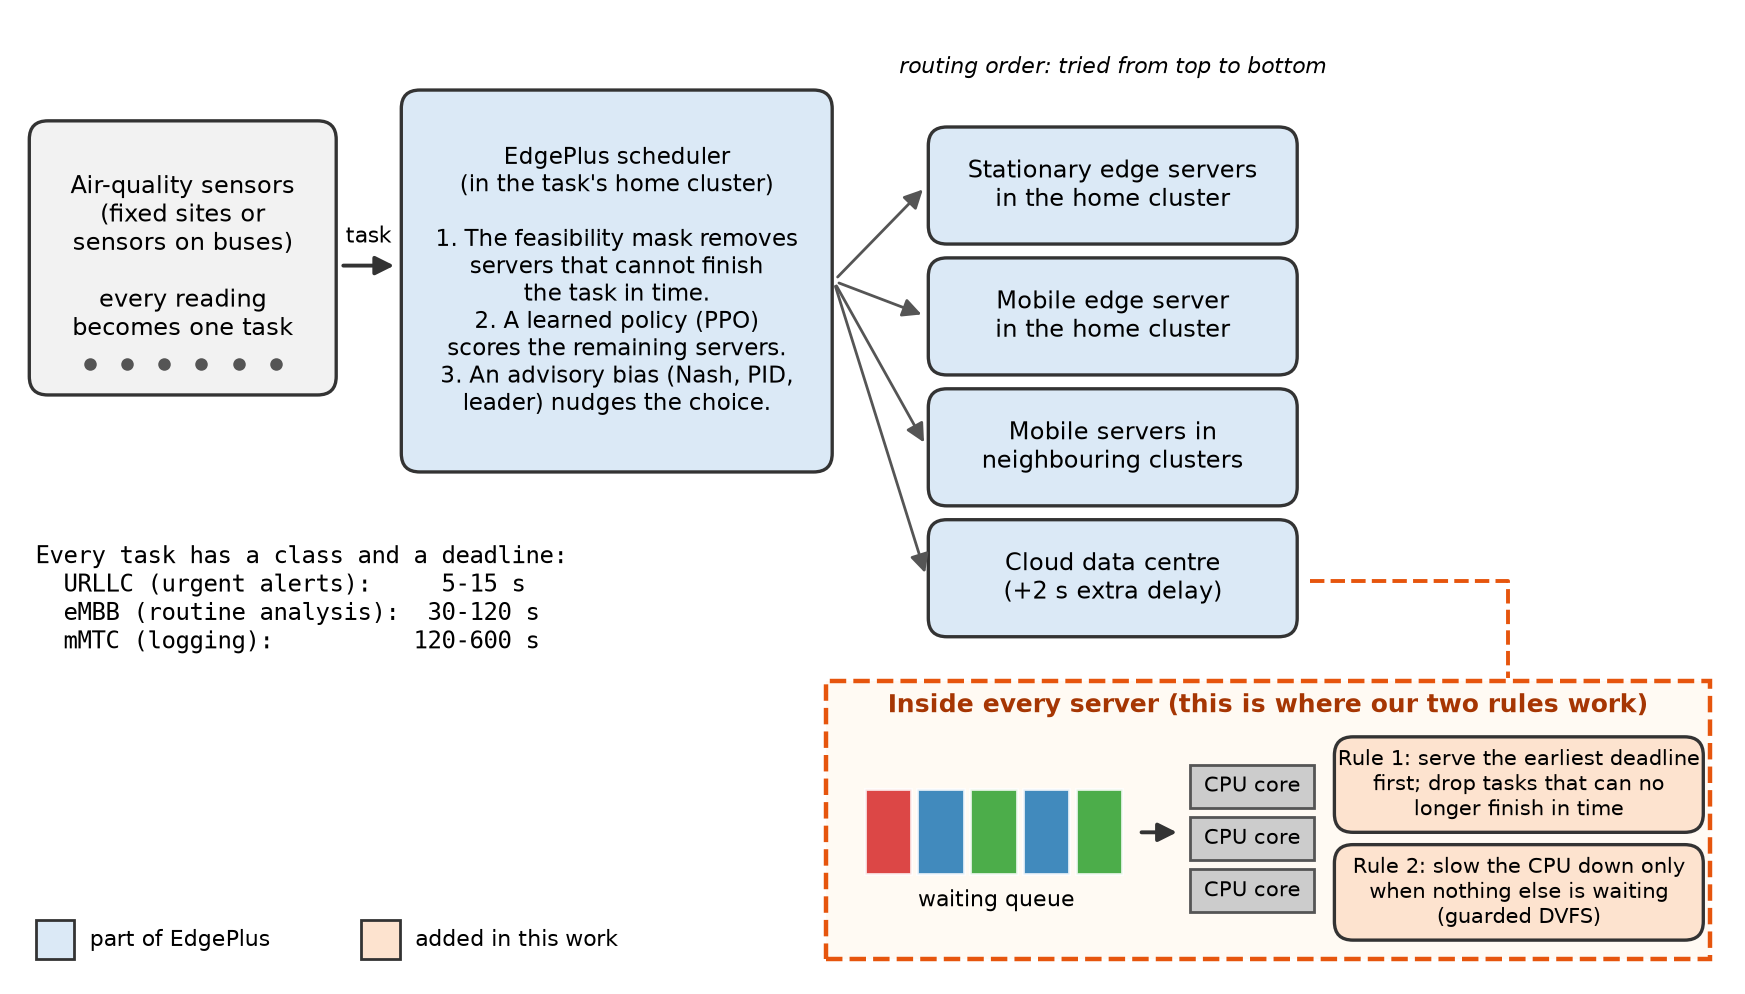
\includegraphics[width=\textwidth]{figures/system_overview.png}
\caption{The system at a glance. A sensor reading becomes a task. EdgePlus (blue) decides which server should run
it. Our two rules (orange) decide, inside each server, which waiting task runs next and how fast the CPU runs.}
\label{fig:overview}
\end{figure}

\paragraph{What we found.} We rebuilt EdgePlus in a computer simulation of a 100\,km$^2$ city, trained it, and
tested it on two datasets: the CityPulse air-quality data used by the EdgePlus authors, and real sensor data
from 13 public buses in Delhi (AirDelhi \cite{airdelhi2023}). The main results are:
\begin{itemize}
\item At heavy load, the share of tasks finished on time rises from 80.5\% to 99.7\% on CityPulse and from
73.0\% to 96.5\% on AirDelhi. Missed urgent tasks fall from 55.4\% to 0.07\% on CityPulse.
\item At light load, energy per task falls by 19.8\% on CityPulse and 11.2\% on AirDelhi, while the share of
tasks finished on time stays the same or improves.
\item The price is a longer wait for relaxed tasks. On CityPulse at heavy load, the 95th-percentile latency of
all tasks rises from 148\,s to 298\,s, but the relaxed tasks still meet their deadlines (only 0.05\% miss).
\item Each design detail matters. Without dropping, without deadline order, with fixed class priorities instead
of deadlines, or without the guard on the slow-down, results are worse.
\end{itemize}

\paragraph{Contributions.} (1) Two server-side rules, one for priority scheduling and one for energy saving,
together with a matching change to EdgePlus's waiting-time estimate. (2) An open rebuild of EdgePlus that we
checked against the numbers in the original paper. (3) A careful evaluation on two datasets, one of them real
measured data, with results per task class, per city area and over time, plus statistical tests.

\paragraph{How to read this paper.} Section~\ref{sec:background} explains all the background ideas from scratch,
with small examples. Section~\ref{sec:edgeplus} describes EdgePlus. Section~\ref{sec:method} presents our two
rules. Section~\ref{sec:setup} describes the simulated city, the data and the experiments, and
Section~\ref{sec:results} the results. Section~\ref{sec:discussion} discusses what the results mean and what
their limits are. Table~\ref{tab:glossary} collects the terms used throughout.



%=====================================================================================================
\section{Background: the ideas you need}
\label{sec:background}
%=====================================================================================================

This section explains, from the beginning, every idea the rest of the paper uses. Table~\ref{tab:glossary}
summarises the most important words; you can come back to it at any time.

\begin{table}[!htbp]
\caption{Words used in this paper.}
\label{tab:glossary}
\small
\begin{tabularx}{\textwidth}{>{\raggedright\bfseries\arraybackslash}p{3.4cm}L}
\toprule
Term & Meaning in this paper\\
\midrule
Task & One piece of computing work created by one sensor reading, for example ``check this reading for a
pollution spike''.\\
Deadline & The time by which a task must finish to be useful. A task that finishes later counts as a miss.\\
On time & Finished before its deadline. The \emph{on-time rate} is the share of all tasks finished on time.\\
Latency & Time from the moment a task is created until it finishes.\\
Slack & How much time a task can still afford to lose: deadline minus the earliest possible finish time.\\
Edge server & A computer near the sensors. Here every edge server has several CPU cores.\\
Cluster & One area of the city with its own group of edge servers. Our city has 10 clusters.\\
Queue & The line of tasks waiting for a free CPU core on a server.\\
FCFS & First come, first served: tasks run in the order they arrived.\\
EDF & Earliest deadline first: the waiting task with the closest deadline runs next.\\
DVFS & Dynamic voltage and frequency scaling: running a CPU slower to save energy.\\
URLLC, eMBB, mMTC & The three 6G service classes, used here for urgent, routine and relaxed tasks.\\
Load & How many tasks arrive in one 10-minute episode: 50{,}000 (light), 100{,}000 (medium) or 150{,}000 (heavy).\\
Episode & One simulated run of 10 minutes of task arrivals, followed by the time needed to finish them.\\
Policy & The learned decision rule inside EdgePlus that picks a server for each task.\\
Feasibility mask & A filter that removes servers that cannot finish a task in time, before the policy chooses.\\
95th percentile & The value that 95\% of measurements are below. ``95th-percentile latency 10\,s'' means 95\% of
tasks finished within 10\,s.\\
\botrule
\end{tabularx}
\end{table}

\subsection{Edge computing and 6G in plain words}
A \emph{cloud data centre} is a large building full of computers, often hundreds or thousands of kilometres away
from the user. It has almost unlimited capacity, but every request has to travel there and back, which adds
delay. \emph{Edge computing} places smaller computers, called edge servers, close to where the data is
produced, for example at a mobile base station in each neighbourhood. They have less capacity than the cloud
but answer much faster.

Each new generation of mobile networks has added new abilities. 5G introduced three kinds of service that 6G
keeps and extends \cite{chaurasia2026}: \emph{ultra-reliable low-latency communication} (URLLC) for urgent
messages, \emph{enhanced mobile broadband} (eMBB) for heavier everyday traffic, and \emph{massive machine-type
communication} (mMTC) for huge numbers of small, delay-tolerant devices. EdgePlus maps air-quality tasks onto
these three classes, and so do we (Table~\ref{tab:classes}).

\begin{table}[!htbp]
\caption{The three task classes. Deadline ranges and shares follow EdgePlus \cite{edgeplus2026}; the average CPU
work is our choice (1 Gcycle = one billion CPU cycles; a 3\,GHz core does three of them per second).}
\label{tab:classes}
\small
\begin{tabularx}{\textwidth}{lLccc}
\toprule
Class & What it stands for in our city & Deadline & Share of tasks & Average CPU work\\
\midrule
URLLC & urgent: a reading that looks like a dangerous pollution spike & 5--15\,s & 20\% & 6 Gcycles\\
eMBB & routine: normal analysis and map updates & 30--120\,s & 50\% & 12 Gcycles\\
mMTC & relaxed: low readings that only need to be logged & 120--600\,s & 30\% & 9 Gcycles\\
\botrule
\end{tabularx}
\end{table}

\subsection{How a server works through its tasks}
An edge server has a few CPU cores. Each core runs one task at a time from start to finish (it does not pause a
task halfway to run another). When all cores are busy, new tasks wait in a \emph{queue}. Whenever a core becomes
free, the server must decide which waiting task to run next. This decision is called \emph{scheduling}, and the
rule used to make it is the \emph{scheduling policy}. Three common ones are:
\begin{itemize}
\item \textbf{First come, first served (FCFS):} the task that has waited longest runs next. It is simple and
fair in one sense, but it ignores deadlines completely. This is what EdgePlus assumes.
\item \textbf{Fixed priority:} every task has a priority class, and the highest class always goes first. For us
that would mean URLLC before eMBB before mMTC.
\item \textbf{Earliest deadline first (EDF):} the waiting task whose deadline comes soonest runs next. EDF is a
kind of priority scheduling in which the priority is the deadline itself, so a relaxed task gradually becomes
more urgent as its deadline approaches.
\end{itemize}

EDF has a famous strength and a famous weakness. The strength: on a single processor that can pause and resume tasks, EDF
meets every deadline as long as the processor is not overloaded \cite{liu1973}, and ordering tasks by deadline also
keeps the worst lateness as small as possible \cite{jackson1955}. The weakness: when there is more work than time
(\emph{overload}), EDF can make things worse than FCFS. It keeps running the task with the closest deadline even
when that task is already doomed, and every task behind it then becomes late too. This chain reaction is known
as the \emph{domino effect} \cite{locke1986,buttazzo2011}. The usual fix is to drop, or skip, tasks that can no
longer make their deadline. Our worked example below shows all three cases.

\begin{workedexample}{1}[why the order of tasks matters]
One server with a single core receives five tasks (all times in seconds):

\begin{center}
\begin{tabular}{cccccc}
\toprule
Task & Class & Arrives at & Needs & Deadline (relative) & Must finish by\\
\midrule
A & mMTC & 0.0 & 4 & 300 & 300.0\\
B & eMBB & 0.5 & 3 & 60 & 60.5\\
C & URLLC & 1.0 & 2 & 8 & 9.0\\
D & URLLC & 1.5 & 2 & 6 & 7.5\\
E & URLLC & 2.0 & 3 & 3 & 5.0\\
\botrule
\end{tabular}
\end{center}

\noindent Task A arrives first and runs from 0 to 4\,s under every rule, because nothing else is waiting yet. At
$t=4$\,s, tasks B, C, D and E are all waiting, and the rules make different choices (Figure~\ref{fig:toy}):
\begin{itemize}
\item \textbf{FCFS} runs them in arrival order B, C, D, E. B and C finish in time, but D finishes at 11\,s
(deadline 7.5) and E at 14\,s (deadline 5). \textbf{3 of 5 on time.}
\item \textbf{EDF without dropping} runs E first because its deadline (5\,s) is the closest. But E needs 3\,s and
cannot finish before 7\,s, so it is late anyway, and while it runs, D and C also become late. \textbf{2 of 5 on
time:} the domino effect makes EDF worse than FCFS.
\item \textbf{EDF with dropping (our Rule~1)} sees at $t=4$\,s that E cannot possibly finish by 5\,s, drops it,
and runs D (4--6\,s), C (6--8\,s) and B (8--11\,s). \textbf{4 of 5 on time.} Task E was lost under every rule;
dropping it early saved the other three.
\end{itemize}
\end{workedexample}

\begin{figure}[!htbp]
\centering
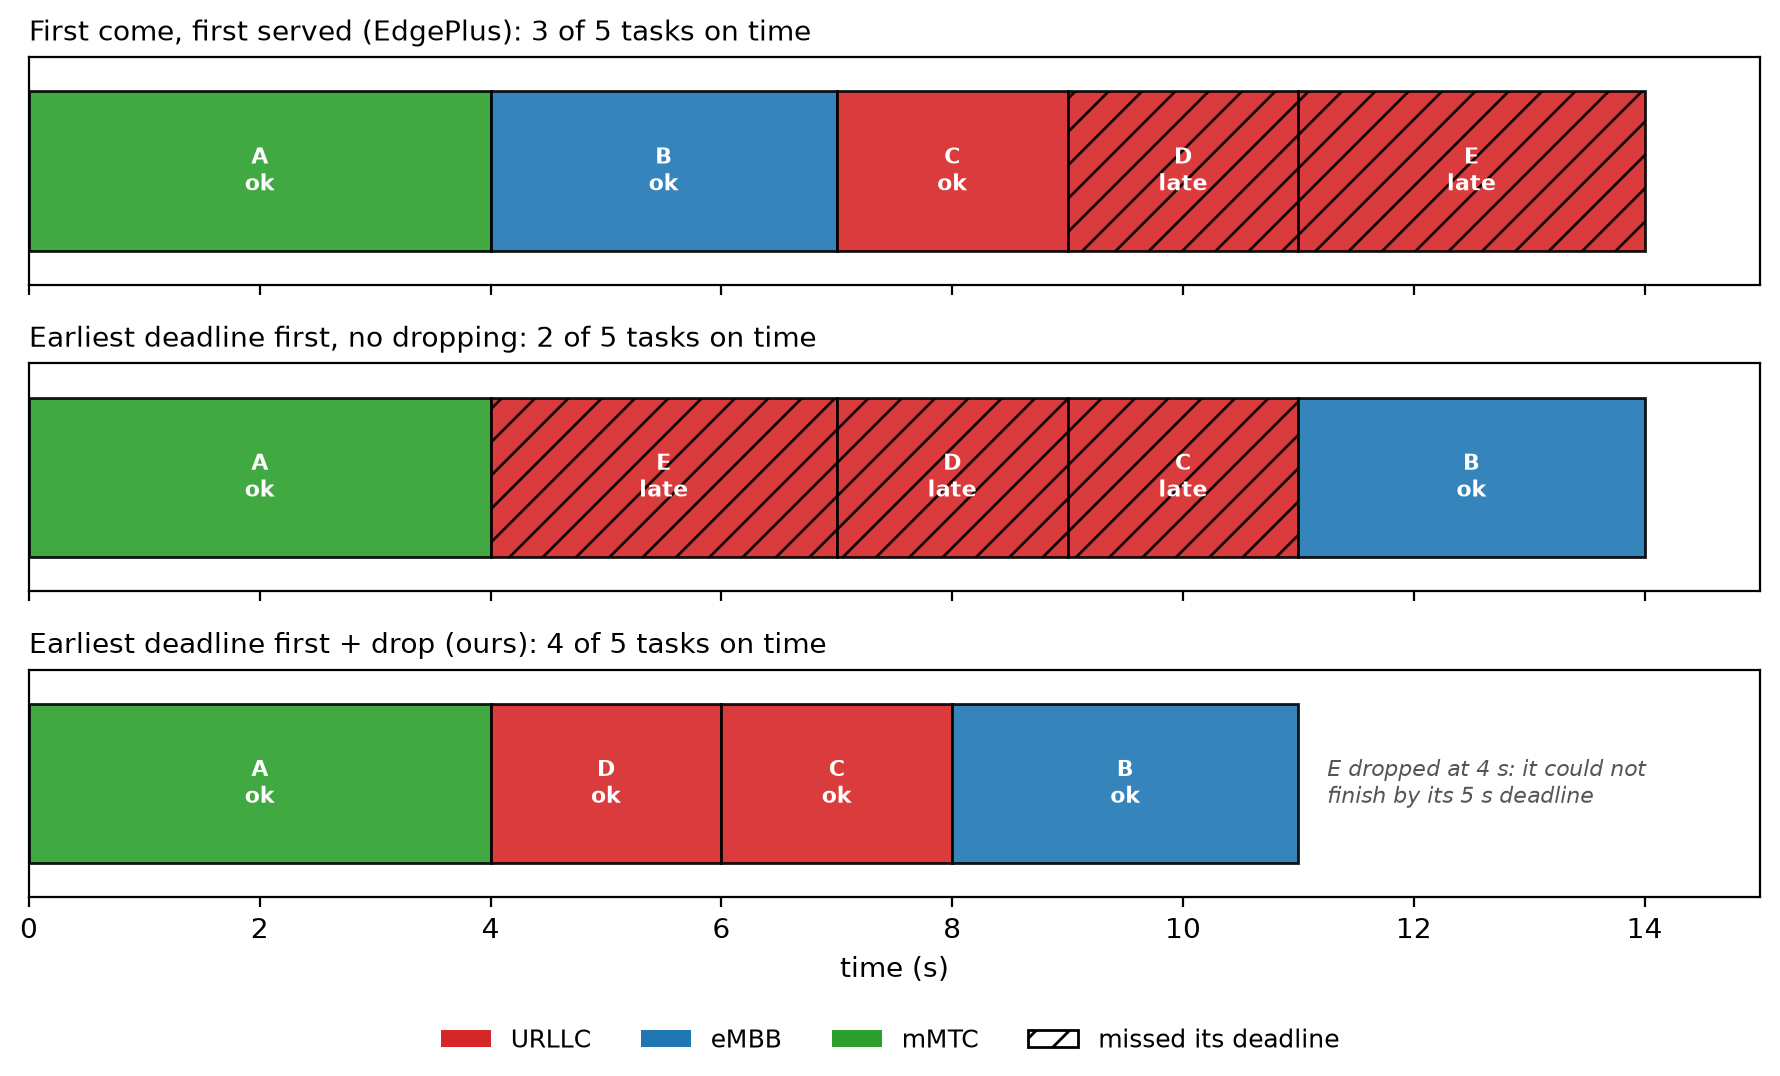
\includegraphics[width=0.92\textwidth]{figures/toy_queue.png}
\caption{Worked example 1 as a timeline. Each bar is a task on the server's single core; hatched bars missed
their deadline.}
\label{fig:toy}
\end{figure}

\subsection{CPU speed and energy}
A processor's power use has two parts. The \emph{dynamic} part is spent on the switching of transistors while
computing. If the clock frequency and the supply voltage are lowered together, dynamic power falls roughly with
the cube of the frequency, so the dynamic energy needed for a fixed amount of work falls roughly with its square.
The \emph{static} part is power drawn just because the chip is switched on and busy; it adds up with running
time, so running slower makes it larger. DVFS, lowering the voltage and frequency when full speed is not needed,
exploits this trade-off and is widely used in phones and servers \cite{weiser1994,pillai2001}.

We model the energy of a task run at a fraction $\phi$ of full speed ($0<\phi\le1$) as
\begin{equation}
E(\phi) = E_{\text{full}} \left(0.75\,\phi^{2} + \frac{0.25}{\phi}\right),
\label{eq:energy}
\end{equation}
where $E_{\text{full}}$ is its energy at full speed, 75\% of which is dynamic and 25\% static. At $\phi = 1$ the
formula gives exactly $E_{\text{full}}$, so the energy of EdgePlus itself is unchanged. Figure~\ref{fig:dvfs}
(left) plots the formula. Slowing down saves energy until about 55\% speed; below that, the extra static energy
outweighs the dynamic saving. Table~\ref{tab:speeds} lists the speeds our rule may choose.

\begin{table}[!htbp]
\caption{The CPU speeds our rule may choose, how much longer a task takes, and how much energy it then needs
(from Equation~\ref{eq:energy}).}
\label{tab:speeds}
\small
\begin{tabular}{lcccccc}
\toprule
Speed (fraction of full) & 100\% & 90\% & 80\% & 70\% & 60\% & 50\%\\
\midrule
Running time & 1.00$\times$ & 1.11$\times$ & 1.25$\times$ & 1.43$\times$ & 1.67$\times$ & 2.00$\times$\\
Energy needed & 1.000 & 0.885 & 0.793 & 0.725 & 0.687 & 0.688\\
Energy saved & 0\% & 11.5\% & 20.8\% & 27.5\% & 31.3\% & 31.2\%\\
\botrule
\end{tabular}
\end{table}

\begin{figure}[!htbp]
\centering
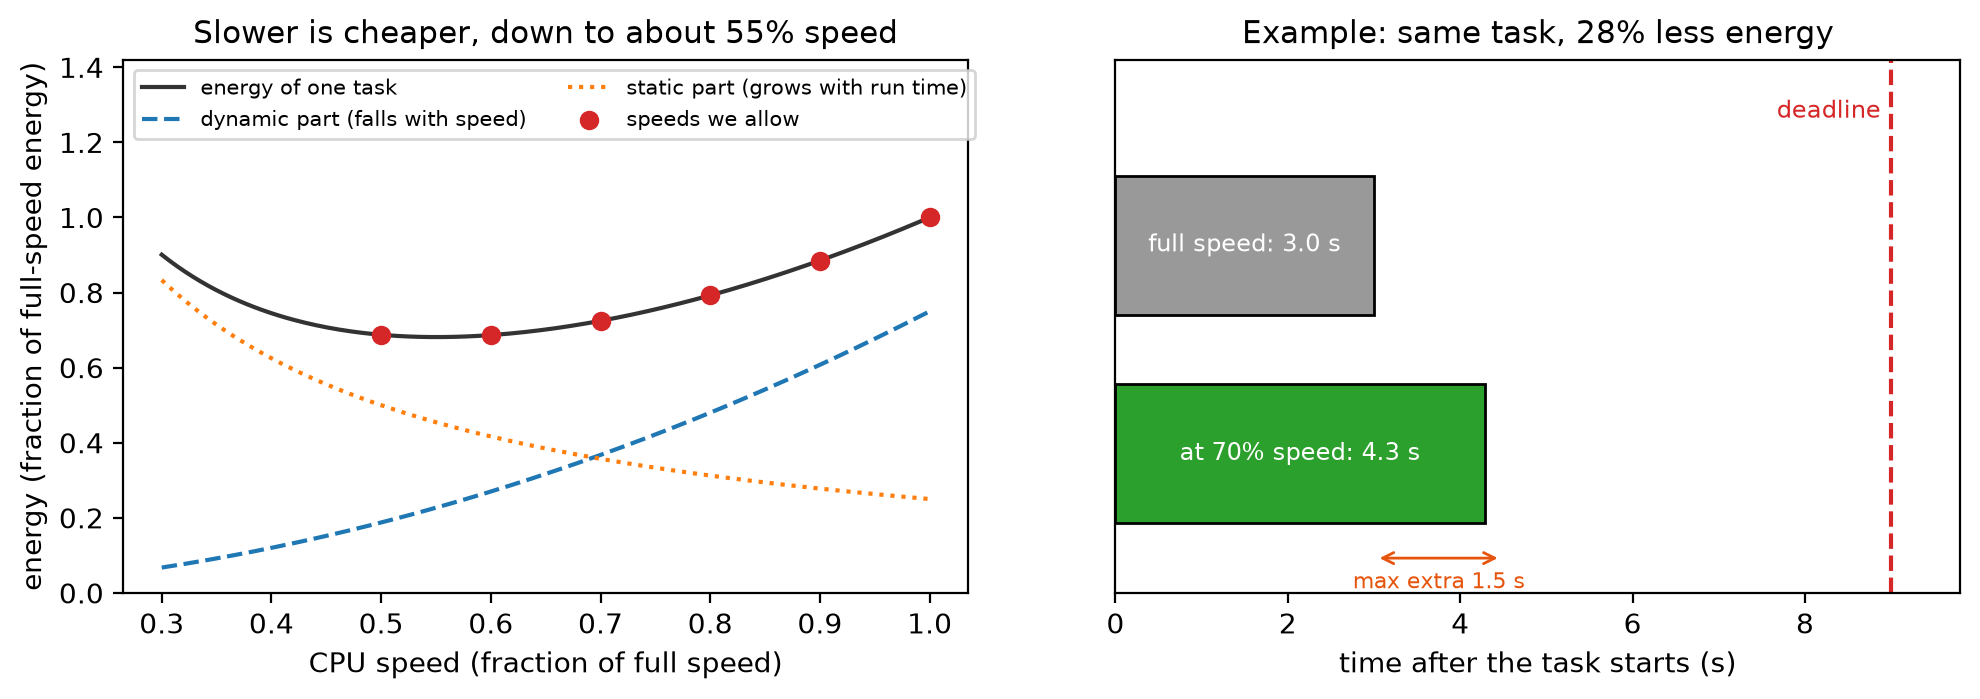
\includegraphics[width=\textwidth]{figures/dvfs_energy.png}
\caption{Left: energy of one task against CPU speed (Equation~\ref{eq:energy}); the dots are the speeds we allow.
Right: worked example 2. A task needing 3\,s at full speed with 6\,s of spare time is run at 70\% speed, takes
4.3\,s and uses 28\% less energy.}
\label{fig:dvfs}
\end{figure}

There is a catch. A slowed-down task holds its CPU core for longer. If an urgent task arrives in the meantime and
all cores are busy, the urgent task has to wait for that longer time. This is why our energy rule comes with a
guard (Section~\ref{sec:rule2}).

\subsection{Reinforcement learning in one page}
Reinforcement learning (RL) is a way for a program, called the \emph{agent}, to learn good decisions by trial and
error. At each step the agent looks at the current situation (the \emph{state}), picks an \emph{action}, and later
receives a \emph{reward}: a number that says how good the outcome was. Over many attempts the agent adjusts its
\emph{policy}, the rule that maps states to actions, so that it collects more reward.

In EdgePlus, a step happens every time a new task arrives:
\begin{itemize}
\item the \textbf{state} describes the task (class, deadline, size) and the candidate servers (how busy they are,
how long the task would wait, how far away they are);
\item the \textbf{action} is the choice of one server;
\item the \textbf{reward} is positive if the task finishes on time and negative if it is late, with smaller
penalties for long latency, high energy, using the cloud and choosing unreliable servers.
\end{itemize}
EdgePlus learns with \emph{proximal policy optimization} (PPO) \cite{schulman2017ppo}, a popular RL method that
improves the policy in small, careful steps so that learning does not become unstable. PPO uses two neural
networks: the \emph{actor}, which gives each candidate server a score, and the \emph{critic}, which estimates how
good the current situation is and helps the actor tell lucky outcomes from good decisions.

\begin{plainwords}[the feasibility mask]
Before the actor scores the servers, EdgePlus removes every server that clearly cannot finish the task in time
(or that is out of memory, battery or reserved capacity). The actor then only chooses among the rest. This is
like a delivery app that hides restaurants which are already closed before you start choosing: you can still
make a poor choice, but never an impossible one. The EdgePlus authors found that this mask was the single most
important part of their design.
\end{plainwords}

\subsection{The statistics used in this paper}
Every number we report is an average over 30 runs: 3 separately trained EdgePlus models $\times$ 10 different
test episodes. To show how certain an average is, we give a \emph{95\% confidence interval} (CI), written
``mean $\pm$ half-width''; roughly, it is the range in which the true average very likely lies. To check whether
a difference is real or just luck, we use \emph{paired} comparisons: the same trained model on the same test
episode is run once with EdgePlus's rules and once with ours, and only the difference matters. The
\emph{Wilcoxon signed-rank test} \cite{wilcoxon1945} turns these 30 differences into a \emph{p-value}, the
probability of seeing differences this consistent if the rules made no difference at all; small values (below
0.05) mean the difference is real. Because we run many tests, we adjust the p-values with the
\emph{Benjamini--Hochberg} method \cite{bh1995}, which keeps the share of false alarms low.

%=====================================================================================================
\section{EdgePlus: the starting point}
\label{sec:edgeplus}
%=====================================================================================================

\subsection{The city and its servers}
EdgePlus \cite{edgeplus2026} models a smart city of 100\,km$^2$ divided into 10 clusters. Each cluster has
stationary edge servers and mobile edge servers (servers mounted on vehicles that can drive to busy areas), and
the whole city shares a cloud data centre. A task is first offered to servers in a fixed \emph{routing order}:
the stationary servers of its own cluster, then the mobile server of its own cluster, then mobile servers in
neighbouring clusters, and finally the cloud. The latency of a task is the sum of four parts: sending the data
(transmission), driving a mobile server closer if needed (movement), waiting in the queue, and computing.

\subsection{How EdgePlus picks a server}
For every task, EdgePlus does three things:
\begin{enumerate}
\item The \textbf{feasibility mask} removes servers that cannot finish the task in time or that would break a
limit: memory, battery of a mobile server, or the capacity reserved for each class (``network slices'').
\item The \textbf{actor network} gives every remaining server a score.
\item An \textbf{advisory layer} adds small bonuses to the scores. A \emph{Nash sharing} rule favours clusters
willing to accept extra work, a \emph{PID controller} (a classic feedback controller) steers each cluster towards
a target utilisation, and \emph{leader election} favours the least-loaded, best-charged server of each cluster.
\end{enumerate}
The task goes to a server picked according to the final scores. EdgePlus also has a \emph{blockchain-lite ledger}:
it records completed tasks, and the record is used to give each server a \emph{reputation} (its recent share of
on-time tasks) and each cluster a \emph{debt} (how far it is below a throughput target). Both enter the state,
the reward and the mask; urgent tasks avoid servers with poor reputation.

\subsection{What EdgePlus reports, and what it leaves open}
EdgePlus also includes a particle swarm optimisation (PSO) outer loop that tunes training, and a security layer
(encryption and signatures). At the heaviest load (150{,}000 tasks) the paper reports 82.77\% of tasks on time,
a median latency of 53.2\,s and a 95th-percentile latency of 147.1\,s; without PSO the on-time rate is 82.0\%.

Three things are left open. First, the queue model that EdgePlus uses to estimate waiting time (Kingman's
formula \cite{kingman1961}) assumes FCFS; nothing gives urgent tasks priority inside a server. The paper does
attach a high/moderate/low priority label to each task, but it is only used to break ties. Second, compute
energy is modelled as a constant times the CPU work, so the CPU always runs at full speed. Third, the paper
defines a URLLC reliability measure but reports results only for all tasks together, so it cannot show which
classes miss their deadlines. Our work addresses all three.

%=====================================================================================================
\section{Our method: two rules inside each server}
\label{sec:method}
%=====================================================================================================

Both rules work inside a server and use the same idea: \emph{slack}, the time a task can still afford to lose.
If a task with deadline $D$ would finish at time $t + w$ when started now at full speed (it needs $w$ seconds),
its slack is
\begin{equation}
\sigma = D - (t + w).
\label{eq:slack}
\end{equation}
A task with small slack is urgent and should go first at full speed. A task with large slack can wait, or can
run more slowly.

\subsection{Rule 1: earliest deadline first, with dropping}
\label{sec:rule1}
Whenever a CPU core becomes free, the server:
\begin{enumerate}
\item looks at all waiting tasks and takes the one with the earliest deadline;
\item checks whether it can still finish in time at full speed, that is, whether its slack $\sigma \ge 0$;
\item if it can, runs it; if it cannot, drops it (it counts as a missed deadline) and goes back to step 1.
\end{enumerate}
Dropping only removes tasks that are already lost: such a task would have missed its deadline under any rule. The
benefit is that the CPU time it would have used goes to tasks that can still be saved, which stops the domino
effect of worked example~1.

\paragraph{Keeping the mask honest.} EdgePlus's mask asks ``how long would this task wait at this server?''.
With FCFS the answer is ``until all the work already queued has been done''. With EDF, a new task only waits for
queued tasks whose deadline is earlier than its own. So we change the estimate to
\begin{equation}
\widehat{W} = r_{\min} + \frac{1}{c}\Bigl(\sum_{\text{queued } j \text{ with } D_j \le D} w_j \; + \; w_{\text{in transit}}\Bigr),
\label{eq:wait}
\end{equation}
where $c$ is the number of cores, $r_{\min}$ is the time until the first busy core becomes free (zero if a core is
free), $w_j$ is the work of a queued task $j$, and $w_{\text{in transit}}$ is work already sent to this server
but not yet arrived. Without this change the mask would keep rejecting busy servers for urgent tasks, even though
EDF would let those tasks jump the queue and finish in time.

\begin{workedexample}{3}[the waiting-time estimate]
A server has 2 cores, both busy for another 1\,s. In its queue are a relaxed task (deadline in 400\,s, needs
6\,s) and a routine task (deadline in 80\,s, needs 4\,s). A new urgent task arrives with a 10\,s deadline.
Under FCFS it would wait $1 + (6+4)/2 = 6$\,s. Under EDF neither queued task has an earlier deadline, so it waits
only $r_{\min} = 1$\,s. With the FCFS estimate the mask might wrongly reject this server; with
Equation~\ref{eq:wait} it correctly accepts it.
\end{workedexample}

\subsection{Rule 2: guarded CPU slow-down}
\label{sec:rule2}
When a task is about to start, the server may run it below full speed, but only if all three conditions hold:
\begin{enumerate}
\item \textbf{nothing else is waiting} for this server and nothing is on its way to it;
\item the extra running time is at most \textbf{80\% of the task's slack}, so it still finishes on time with a
margin;
\item the extra running time is at most \textbf{1.5 seconds} (the guard).
\end{enumerate}
Among the allowed speeds $\{50\%, 60\%, \dots, 100\%\}$ the server picks the lowest one that satisfies these
conditions. Written as a formula, it picks the smallest $\phi$ with
\begin{equation}
\frac{w}{\phi} - w \;\le\; \Delta, \qquad
\Delta = \begin{cases}\min(0.8\,\sigma,\; 1.5\,\text{s}) & \text{if nothing is waiting,}\\
0 & \text{otherwise.}\end{cases}
\label{eq:dvfs}
\end{equation}

Why the guard? Conditions 2 and 3 protect the task itself and the tasks that might arrive while it runs. Without
condition 1 and the 1.5\,s cap, a relaxed task with 300\,s of slack could be slowed to half speed, doubling its
running time. An urgent task arriving a moment later could then find every core occupied by slow tasks. We test
exactly this ``unguarded'' version in Section~\ref{sec:ablation} and it performs very badly.

\begin{workedexample}{2}[slowing down safely]
A task needs 3\,s at full speed and has 6\,s of slack, and nothing else is waiting. The allowed extra time is
$\min(0.8 \times 6,\ 1.5) = 1.5$\,s. At 70\% speed the task takes $3/0.7 = 4.3$\,s, only 1.3\,s extra, so 70\% is
allowed; 60\% would take 5.0\,s, 2\,s extra, which is too much. So the server runs it at 70\% speed. From
Table~\ref{tab:speeds}, it needs 0.725 of the full-speed energy: \textbf{27.5\% less energy}, and it still
finishes 4.7\,s before its deadline (Figure~\ref{fig:dvfs}, right).
\end{workedexample}

\subsection{The complete procedure}
Algorithm~\ref{alg:rules} combines the two rules. It runs every time a core of a server becomes free, and also
when a task reaches a server that has a free core.

\begin{algorithm}[!htbp]
\caption{What a server does when a CPU core becomes free at time $t$}
\label{alg:rules}
\begin{algorithmic}[1]
\While{the queue is not empty}
  \State take the waiting task $i$ with the earliest deadline $D_i$ \Comment{Rule 1: EDF}
  \State $\sigma \gets D_i - t - w_i$ \Comment{slack at full speed}
  \If{$\sigma < 0$}
     \State drop task $i$ (count it as missed) and \textbf{continue} \Comment{Rule 1: drop}
  \EndIf
  \If{the queue is empty and nothing is in transit} $\Delta \gets \min(0.8\sigma, 1.5\,\text{s})$
  \Else\ $\Delta \gets 0$
  \EndIf
  \State $\phi \gets$ the lowest allowed speed with $w_i/\phi - w_i \le \Delta$ \Comment{Rule 2: guarded DVFS}
  \State run task $i$ on the free core at speed $\phi$ and \textbf{stop}
\EndWhile
\end{algorithmic}
\end{algorithm}

\subsection{Why the two rules fit together, and what they cost}
Both rules follow the same logic: urgent tasks (small slack) go first and run at full speed; relaxed tasks
(large slack) wait or run slower. Rule~1 improves the on-time rate when servers are busy, which is exactly when
Rule~2 rarely acts because queues are rarely empty. When servers are quiet, Rule~1 changes little and Rule~2 saves
energy. So the two rules help at different loads without getting in each other's way.

Neither rule needs training. The extra work per decision is small: sorting the queue by deadline and checking a
few speeds. In our simulator, a whole episode including the simulation itself takes 0.23\,ms per task with
EdgePlus's rules and 0.30\,ms with ours, on one CPU core.

%=====================================================================================================
\section{How we tested the idea}
\label{sec:setup}
%=====================================================================================================

\subsection{The simulated city}
We wrote a simulator in Python that follows EdgePlus's description: a 10\,km $\times$ 10\,km city with 10 clusters,
each with 4 stationary edge servers and 1 mobile edge server, plus one cloud. The simulator is \emph{event
driven}: it jumps from one event to the next (a task arrives, a task finishes, a mobile server reaches a new
area), so it can process 150{,}000 tasks in under a minute. Table~\ref{tab:servers} lists the servers.

\begin{table}[!htbp]
\caption{The servers in the simulated city.}
\label{tab:servers}
\small
\begin{tabularx}{\textwidth}{lcL}
\toprule
Server type & How many & Details\\
\midrule
Stationary edge server & 4 per cluster (40) & 24 cores each, at 2.4, 3.0, 3.6 and 3.0\,GHz; 64\,GB memory; placed
around the cluster centre\\
Mobile edge server & 1 per cluster (10) & 16 cores at 2.4\,GHz; 32\,GB memory; drives at 15\,m/s; 2\,km radio range;
2\,kJ battery; can move to an overloaded neighbouring cluster every 20\,s\\
Cloud data centre & 1 & 32 cores at 3.5\,GHz; 2\,s extra delay for sending data there and back\\
\botrule
\end{tabularx}
\end{table}

How do we know where the clusters are? Like EdgePlus, we group the sensor locations with \emph{weighted
K-means}, a standard method that places 10 centres so that every sensor is close to one of them; sensors with
higher pollution readings count a little more. Clusters whose centres are next to each other (found with a
Delaunay triangulation) are \emph{neighbours} and may share their mobile servers. Figure~\ref{fig:topology}
shows the result for both datasets.

\begin{figure}[!htbp]
\centering
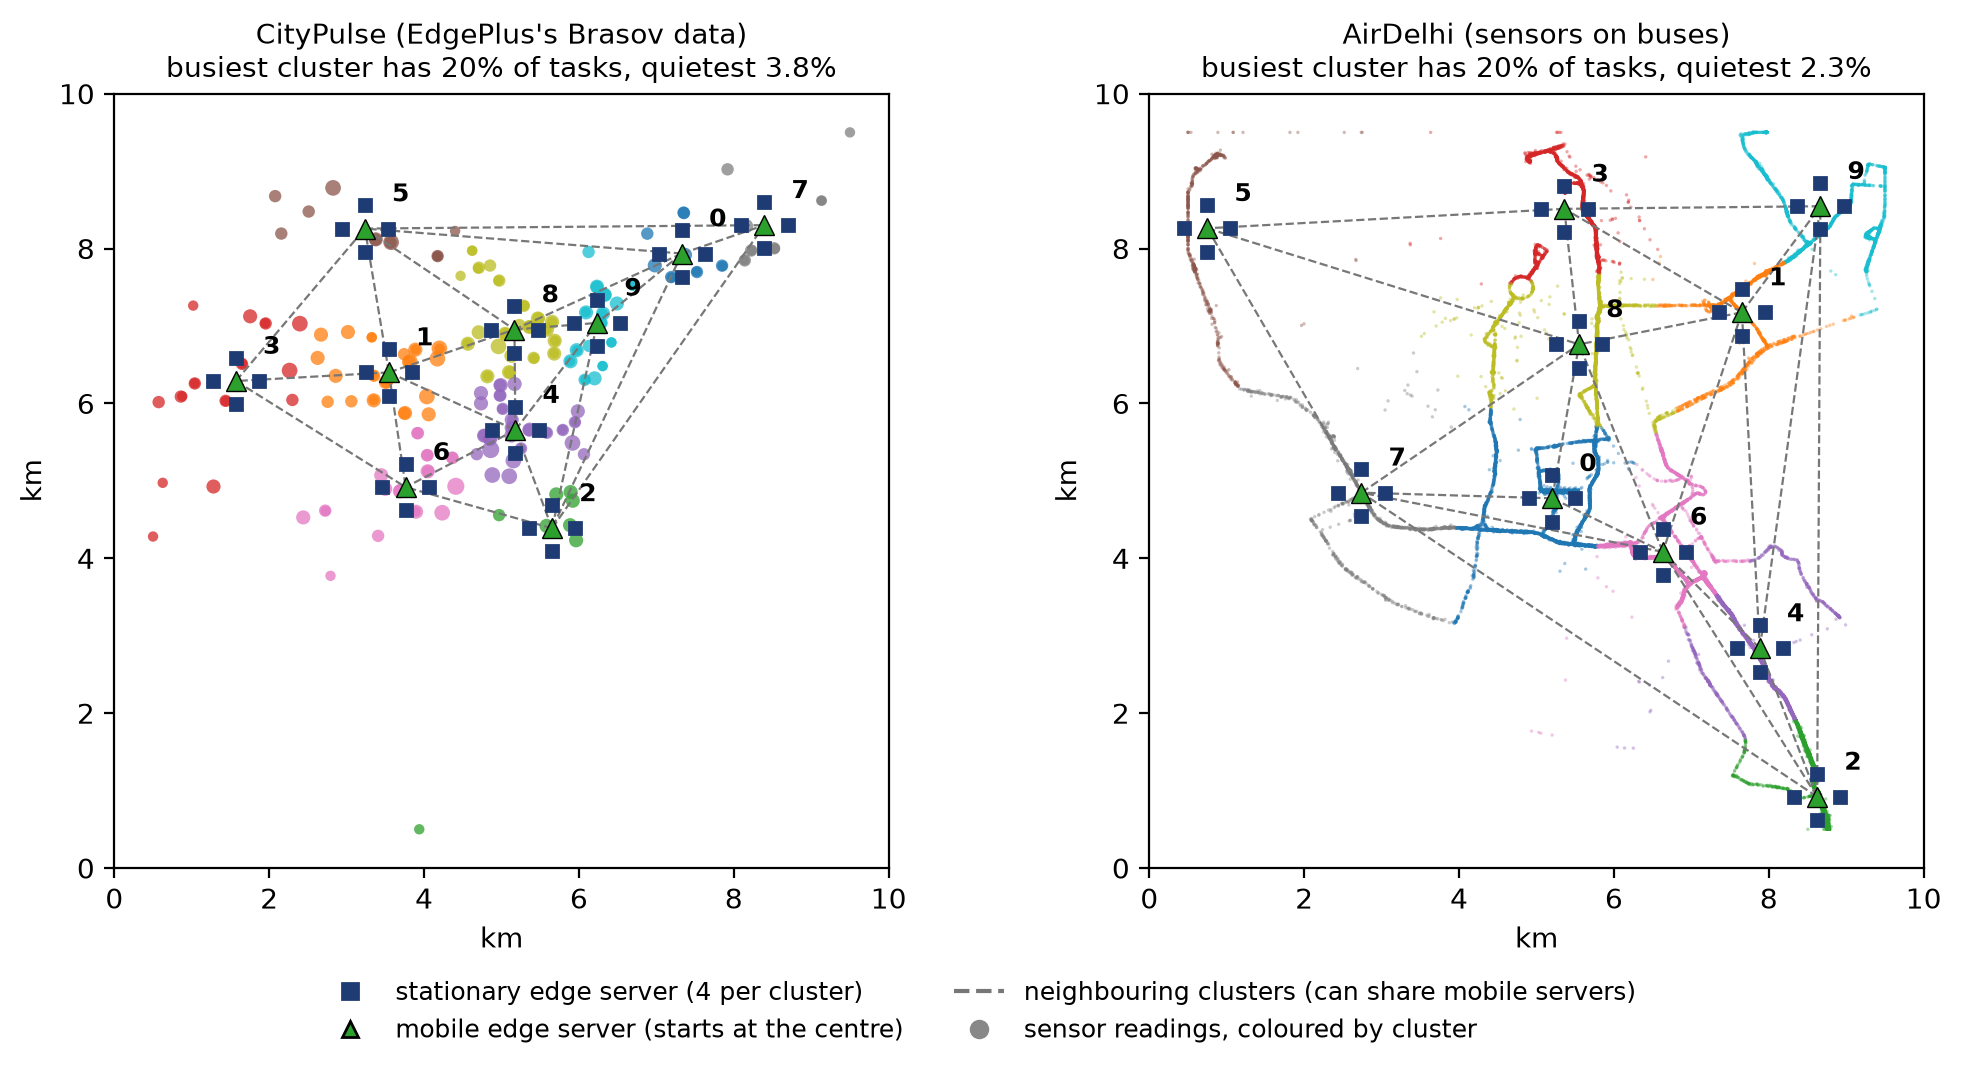
\includegraphics[width=\textwidth]{figures/topology.png}
\caption{The two simulated cities. Coloured dots are sensor locations (left) or bus positions (right), coloured
by cluster; numbers are cluster IDs; dashed lines join neighbouring clusters. Both cities use the same server
inventory, but tasks are spread very unevenly: the busiest cluster receives about 20\% of all tasks in both
cities, and the quietest only 2--4\%.}
\label{fig:topology}
\end{figure}

\subsection{The two datasets}
Table~\ref{tab:datasets} compares the two datasets.

\textbf{CityPulse} \cite{citypulse} is the dataset that EdgePlus calls the Bra\c{s}ov air-pollution traces: 449
sensor sites reporting five pollution values every five minutes from 1 August to 1 October 2014, 7.89 million
readings in total. Two details are worth knowing. The download file on the CityPulse website is named after the
city of Aarhus, and CityPulse describes the values as \emph{generated}: they follow a bounded random walk rather
than real measurements. Also, all sites report at the same moments; we spread each site's reports over its
five-minute interval, and tasks then arrive at a perfectly steady rate.

\textbf{AirDelhi} \cite{airdelhi2023} is real measured data, released by IIT Delhi in 2023: low-cost particulate
matter (PM$_1$, PM$_{2.5}$, PM$_{10}$) sensors mounted on 13 public buses, recording every 3 seconds together with
GPS position. We use December 2020 and January 2021. We removed readings with impossible positions or values,
and readings taken while a bus was standing still (it moved less than 50\,m in about 3 minutes). Without this
step, 38\% of all readings came from just three 1\,km$^2$ squares, mostly from buses standing still, probably at
depots. This left 4.04 million readings. Because buses move between areas and their activity changes through the
day, AirDelhi tasks arrive in strong bursts (Figure~\ref{fig:workload}).

\begin{table}[!htbp]
\caption{The two datasets.}
\label{tab:datasets}
\small
\begin{tabularx}{\textwidth}{lLL}
\toprule
 & CityPulse (EdgePlus's ``Bra\c{s}ov'') & AirDelhi\\
\midrule
Source & CityPulse project, University of Surrey & IIT Delhi, NeurIPS 2023 Datasets track\\
Sensors & 449 fixed sites (208 distinct locations) & 13 sensors on public buses\\
Period used & 1 Aug -- 1 Oct 2014 & 1 Dec 2020 -- 30 Jan 2021\\
Values & 5 pollution indices (ozone, particles, CO, SO$_2$, NO$_2$) & PM$_{2.5}$ and PM$_{10}$ concentrations\\
Real or generated & generated (bounded random walk) & real measurements\\
Readings used & 7.89 million & 4.04 million (after removing parked-bus readings)\\
Training / test split & first 43 days / last 18 days & December / January\\
Arrival pattern & perfectly steady & bursty: from 6 to 455 tasks per second at heavy load\\
\botrule
\end{tabularx}
\end{table}

\subsection{From sensor readings to tasks}
Following EdgePlus's labelling procedure, every reading becomes one task:
\begin{enumerate}
\item \textbf{Severity.} For each pollutant we measure how unusual the reading is compared with the training
period (a robust z-score), and how fast it is rising. The severity of the reading is its most unusual pollutant
plus half of its fastest rise.
\item \textbf{Class.} Within each episode, the 20\% most severe readings become URLLC tasks, the next 50\% eMBB and
the remaining 30\% mMTC, matching EdgePlus.
\item \textbf{Deadline.} Drawn at random from the class's range in Table~\ref{tab:classes}.
\item \textbf{Size.} The CPU work is drawn around the class average, a little higher for more severe readings.
\item \textbf{Home cluster.} The cluster whose centre is closest to the sensor (or to the bus at that moment).
\item \textbf{Arrival time.} An episode takes $N$ consecutive readings and squeezes their real time span into a
10-minute window. $N$ is 50{,}000, 100{,}000 or 150{,}000, giving on average 83, 167 or 250 new tasks per second.
At 150{,}000 tasks an episode covers about 28 hours of CityPulse data or 43 hours of AirDelhi data.
\end{enumerate}

\begin{figure}[!htbp]
\centering
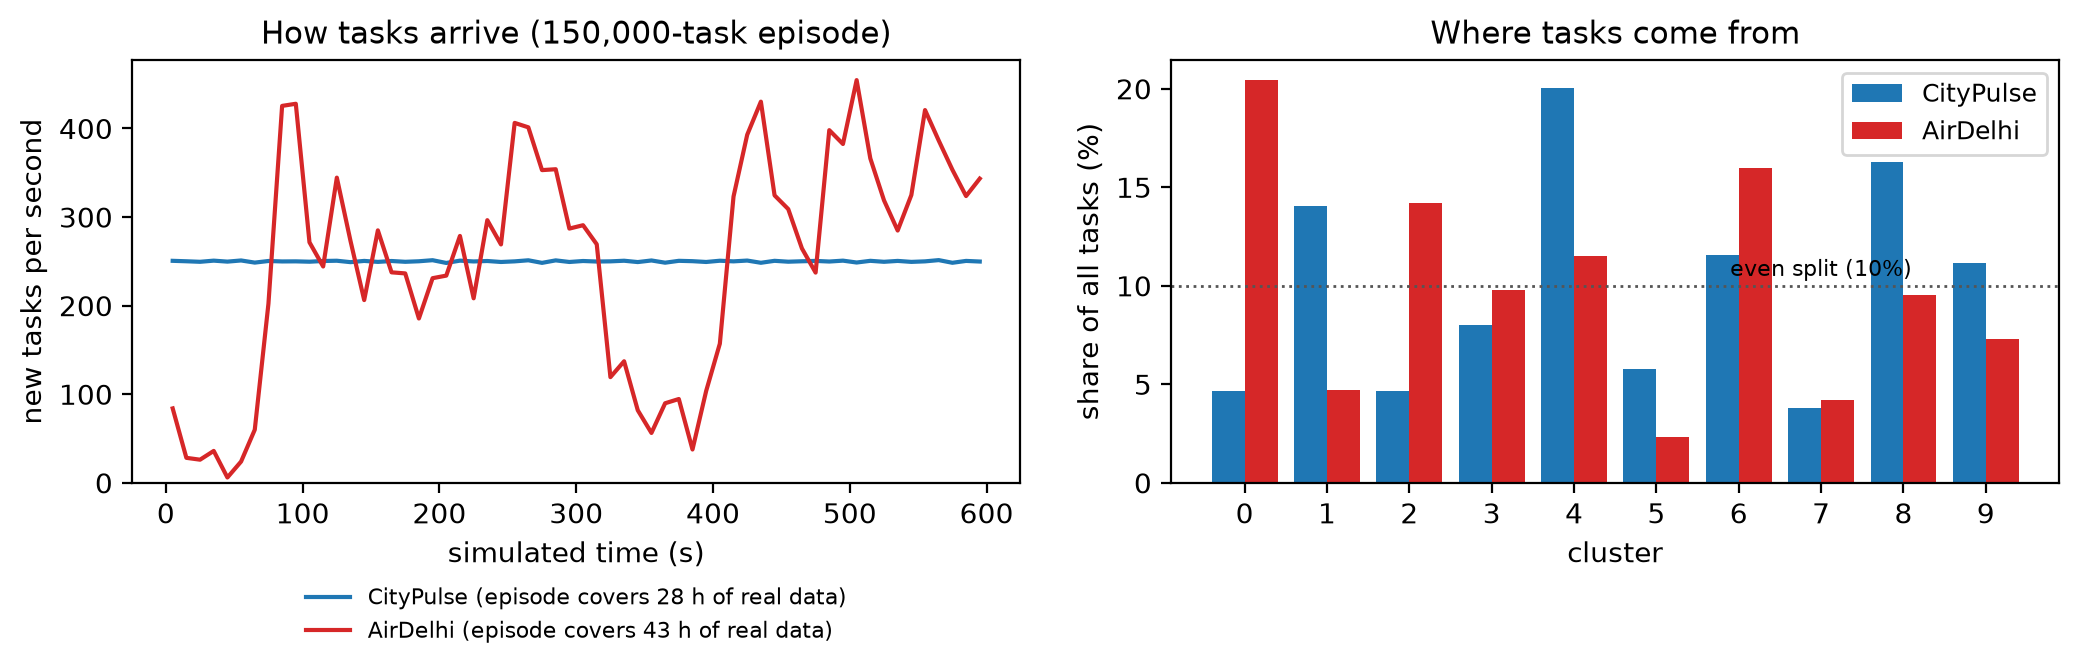
\includegraphics[width=\textwidth]{figures/workload.png}
\caption{The workload. Left: new tasks per second during one heavy-load test episode; CityPulse is perfectly
steady, AirDelhi is bursty. Right: share of all tasks coming from each cluster.}
\label{fig:workload}
\end{figure}

\subsection{Rebuilding EdgePlus}
We could not find public code for EdgePlus, so we rebuilt it from the paper. Table~\ref{tab:rebuild} shows what we kept and
what we simplified. Two simplifications matter most. We left out PSO, so our baseline corresponds to the
paper's ``EdgePlus without PSO'' variant. And we left out the encryption and blockchain machinery, but kept the
reputation and debt signals that the ledger feeds into the scheduler; the ledger's own check takes 0.39\,ms
according to the paper and happens after a task finishes, so it does not affect latency. All other parameter
values are listed in Appendix~\ref{app:params}.

\begin{table}[!htbp]
\caption{What we rebuilt from EdgePlus. Everything here applies equally to the baseline and to our rules.}
\label{tab:rebuild}
\small
\begin{tabularx}{\textwidth}{lL}
\toprule
EdgePlus part & In our rebuild\\
\midrule
Feasibility mask, routing order, slices & Kept: deadline, memory, battery, slice budget and URLLC reputation checks\\
PPO actor and centralised critic & Kept: one actor network shared by all clusters that scores each candidate
server; a critic that sees the whole city\\
Advisory layer (Nash, PID, leader) & Kept, with EdgePlus's PID settings (1.90, 1.20, 0.06)\\
Reward & Kept: on-time bonus, late penalty, latency, energy, cloud, reputation and debt terms\\
Reputation and debt from the ledger & Kept as signals; the blockchain itself is not simulated\\
Waiting-time estimate & Uses the server's real queue instead of Kingman's formula (more accurate for the
baseline too)\\
Servers & Multi-core servers, simulated task by task\\
Mobile server paths & Straight line $\times$ 1.3 (instead of CBS--D* Lite path planning)\\
PSO outer loop & Not included (baseline = EdgePlus without PSO)\\
Encryption, signatures, security tests & Not included (no effect on scheduling)\\
\botrule
\end{tabularx}
\end{table}

We calibrated one number: the number of cores per stationary server. We chose 24 because the trained EdgePlus
model then comes close to the paper's heavy-load result (80.5\% on time against 82.0\%), while every task is on
time at light load, as in the paper.

\subsection{Training the EdgePlus model}
We trained one EdgePlus model for each load and each of 3 random seeds (9 models). Each model trained for 60
rounds; in each round it simulated one full training episode, collected one decision per task, and updated its
networks with PPO. Training took 25, 45 and 61 minutes per model on one CPU core at the three loads, 6.6
CPU-hours in total. No graphics card was needed, because the networks are small and the simulator does most of
the work.

Figure~\ref{fig:training} shows learning. At light and medium load the model quickly reaches almost 100\% on
time. At heavy load the on-time rate during training climbs from about 74.6\% in the first ten rounds to 79.4\%
in the last ten. (During training the model tries random choices on purpose, so its score is lower than in the
tests, where it always takes its best choice.) The spikes come from training episodes that happened to be
easier. As a check that learning helped, the trained model beats a simple non-learning scheduler at heavy load by
8.5 points (80.5\% against 72.0\% on time).

\begin{figure}[!htbp]
\centering
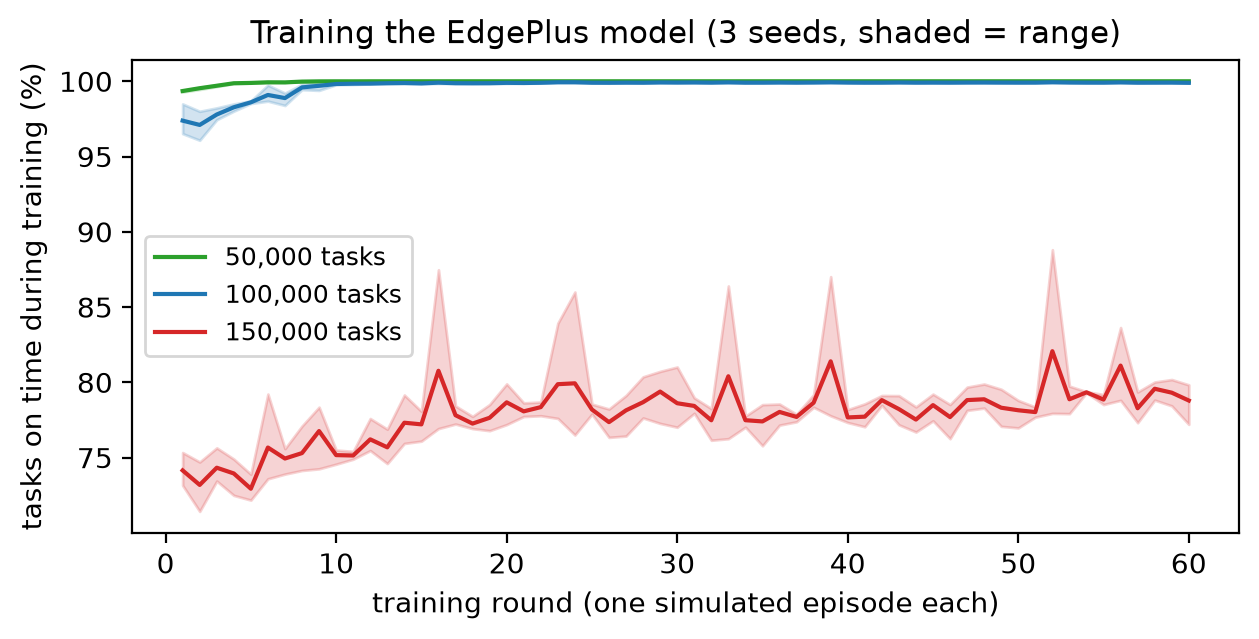
\includegraphics[width=0.72\textwidth]{figures/training.png}
\caption{Training the EdgePlus model: share of tasks on time in each training round (line: average of 3 seeds;
shaded: range).}
\label{fig:training}
\end{figure}

\subsection{The experiments}
Each of the 9 trained models was tested on 10 test episodes taken from the test period of the data, giving 30
runs per setting. In every test we ran the same model with the different server rules listed in
Table~\ref{tab:variants}. For AirDelhi we used the models trained on CityPulse without retraining them, which
also tests how well everything carries over to a new city with real data. Table~\ref{tab:metrics} explains the
measurements.

\begin{table}[!htbp]
\caption{The server rule sets we compared. The first is EdgePlus as published; the last is our full method.}
\label{tab:variants}
\small
\begin{tabularx}{\textwidth}{@{}lLlL@{}}
\toprule
Name & Queue order & Late tasks & CPU speed\\
\midrule
EdgePlus (baseline) & FCFS & kept & always full speed\\
Drop late tasks only & FCFS & dropped & always full speed\\
Deadline first only & EDF & kept & always full speed\\
Fixed class priority + drop & URLLC, then eMBB, then mMTC & dropped & always full speed\\
Rule 1: deadline first + drop & EDF & dropped & always full speed\\
Unguarded slow-down & FCFS & kept & slowed whenever the task has slack\\
Rule 2: guarded slow-down & FCFS & kept & guarded DVFS (Section~\ref{sec:rule2})\\
Both rules (ours) & EDF & dropped & guarded DVFS\\
\botrule
\end{tabularx}
\end{table}

\begin{table}[!htbp]
\caption{What we measure.}
\label{tab:metrics}
\small
\begin{tabularx}{\textwidth}{lL}
\toprule
Measurement & Meaning\\
\midrule
On time (\%) & Share of all tasks that finished before their deadline. Dropped tasks count as missed.\\
Missed (\%) per class & Share of URLLC, eMBB or mMTC tasks that missed their deadline.\\
Median latency & Half of the finished tasks took less than this.\\
95th-percentile latency & 95\% of the finished tasks took less than this; a measure of the slowest tasks.\\
Energy per task & Average energy used per task, in millijoules (mJ), including transmission and computing.\\
Cloud share & Share of tasks sent to the cloud.\\
Dropped (\%) & Share of tasks dropped by Rule 1 (already included in ``missed'').\\
\botrule
\end{tabularx}
\end{table}

%=====================================================================================================
\section{Results}
\label{sec:results}
%=====================================================================================================

\subsection{Is our EdgePlus close to the original?}
Before improving EdgePlus we checked that our rebuild behaves like the original (Table~\ref{tab:fidelity}). At
light load both reach 100\% on time with latencies of a few seconds. At heavy load ours reaches 80.5\% on time
against 82.0\% for the published EdgePlus without PSO, with nearly the same 95th-percentile latency (148\,s
against 147--159\,s). Our median latency and cloud share are lower. The one clear difference is the medium load,
where the paper reports 82.5\% and we measure 99.9\%. The steady arrivals of the CityPulse data leave the servers
far from full at medium load in our simulator. AirDelhi, whose arrivals are bursty, does produce a congested
medium load, so it covers this case.

\begin{table}[!htbp]
\caption{Our rebuilt EdgePlus against the published numbers (CityPulse data).}
\label{tab:fidelity}
\footnotesize
\begin{tabular*}{\textwidth}{@{\extracolsep\fill}llrrrr@{}}
\toprule
Load & Source & On time (\%) & Median (s) & 95th pct (s) & Cloud (\%)\\
\midrule
50{,}000 & EdgePlus paper & 100.00 & 3.98 & 10.24 & --\\
 & our rebuild & 100.00 & 3.55 & 7.35 & 0.00\\
\midrule
100{,}000 & EdgePlus paper & 82.50 & -- & about 151 & --\\
 & our rebuild & 99.87 & 4.20 & 11.79 & 0.09\\
\midrule
150{,}000 & EdgePlus paper & 82.77 & 53.23 & 147.09 & 6.1\\
 & EdgePlus paper, without PSO & 82.0 & 54.8 & 158.9 & 6.6\\
 & our rebuild (without PSO) & 80.52 & 27.95 & 148.10 & 3.78\\
 & simple scheduler, no learning & 71.99 & 38.39 & 125.01 & 3.79\\
\botrule
\end{tabular*}
\end{table}

\subsection{Main result on CityPulse}
Table~\ref{tab:main_cp} and Figure~\ref{fig:main_cp} compare EdgePlus with our rules on the dataset used by the
EdgePlus authors.

At \textbf{heavy load}, Rule~1 raises the share of tasks on time from 80.5\% to 99.6\%. Missed URLLC tasks fall
from 55.4\% to 0.07\% and missed eMBB tasks from 16.8\% to 0.65\%, while mMTC tasks stay almost perfect (0.05\%
missed). Only 0.36\% of tasks are dropped. The median latency drops from 28\,s to under 6\,s. In other words, the
servers had enough capacity all along; under FCFS they were spending it on the wrong tasks first.

At \textbf{light load}, every task is on time with or without our rules, so Rule~1 has nothing to fix. Here
Rule~2 does the work: energy per task falls from 27.04\,mJ to 21.69\,mJ, a saving of 19.8\%. The saving shrinks as
load grows (10.0\% at medium, 5.2\% at heavy load) because busy servers rarely have an empty queue, which is when
Rule~2 is allowed to act. The cost at light load is about one extra second of latency (median 3.6\,s to 4.7\,s),
well within every deadline.

\begin{table}[!htbp]
\caption{CityPulse: EdgePlus with and without our rules (average of 30 runs; the 95\% confidence intervals are
small, for example $\pm0.50$ for EdgePlus's 80.52\% and $\pm0.10$ for our 99.65\%).}
\label{tab:main_cp}
\footnotesize\setlength{\tabcolsep}{4pt}
\begin{tabular*}{\textwidth}{@{\extracolsep\fill}llrrrrrrr@{}}
\toprule
 & & On time & \multicolumn{3}{c}{Missed (\%)} & Median & 95th pct & Energy\\
\cmidrule(lr){4-6}
Load & Rules & (\%) & URLLC & eMBB & mMTC & latency (s) & latency (s) & (mJ/task)\\
\midrule
\multirow{4}{*}{50{,}000} & EdgePlus & 100.00 & 0.00 & 0.00 & 0.00 & 3.55 & 7.35 & 27.04\\
 & + Rule 1 & 100.00 & 0.00 & 0.00 & 0.00 & 3.55 & 7.35 & 27.04\\
 & + Rule 2 & 99.99 & 0.04 & 0.00 & 0.00 & 4.73 & 8.24 & 21.76\\
 & + both (ours) & 100.00 & 0.01 & 0.00 & 0.00 & 4.72 & 8.19 & \textbf{21.69}\\
\midrule
\multirow{4}{*}{100{,}000} & EdgePlus & 99.87 & 0.66 & 0.00 & 0.00 & 4.20 & 11.79 & 27.61\\
 & + Rule 1 & 99.99 & 0.04 & 0.00 & 0.00 & 3.82 & 9.72 & 27.59\\
 & + Rule 2 & 99.84 & 0.79 & 0.00 & 0.00 & 5.05 & 12.39 & 24.83\\
 & + both (ours) & \textbf{99.99} & 0.04 & 0.00 & 0.00 & 4.59 & 10.48 & \textbf{24.86}\\
\midrule
\multirow{4}{*}{150{,}000} & EdgePlus & 80.52 & 55.36 & 16.80 & 0.03 & 27.95 & 148.10 & 28.36\\
 & + Rule 1 & 99.64 & 0.07 & 0.65 & 0.05 & 5.46 & 290.63 & 28.07\\
 & + Rule 2 & 79.60 & 57.11 & 17.94 & 0.04 & 29.81 & 155.12 & 27.11\\
 & + both (ours) & \textbf{99.65} & 0.07 & 0.64 & 0.05 & 5.99 & 298.37 & \textbf{26.88}\\
\botrule
\end{tabular*}
\end{table}

\begin{figure}[!htbp]
\centering
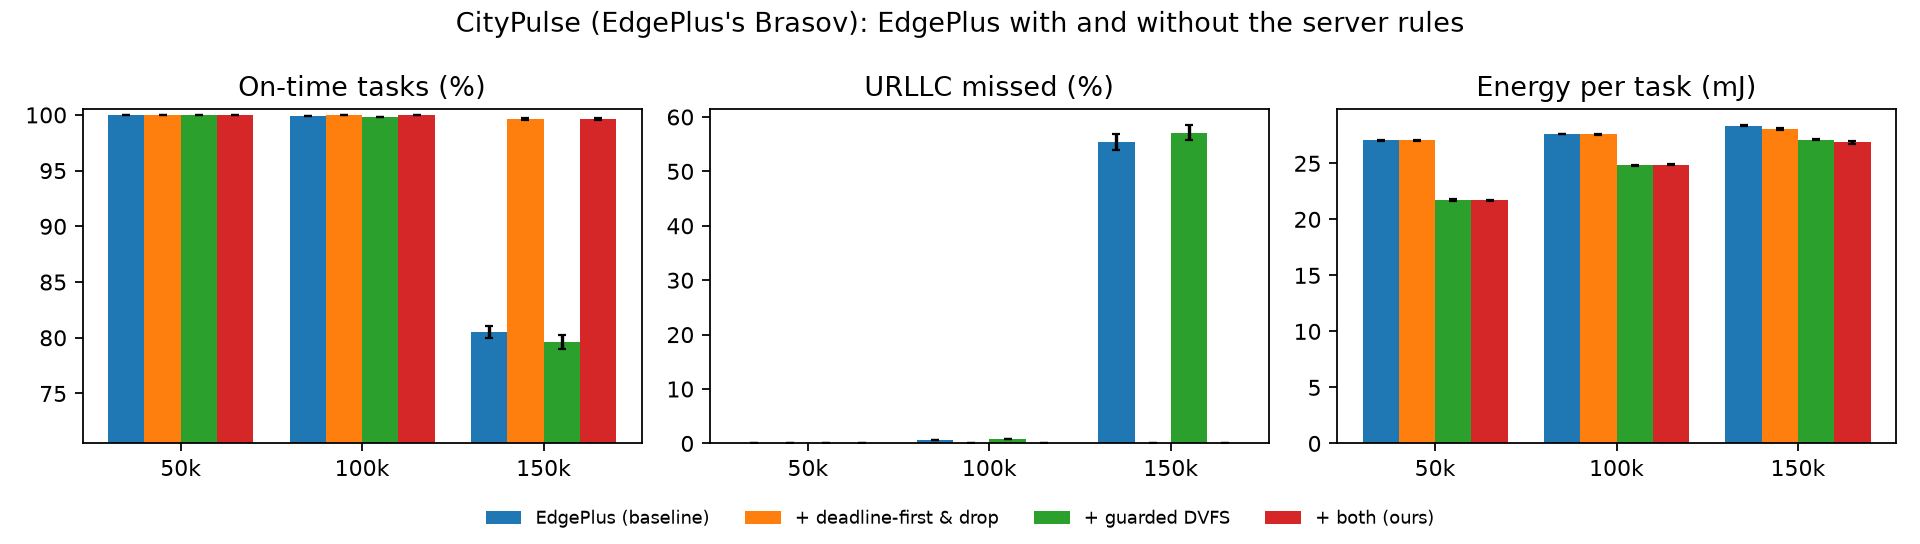
\includegraphics[width=\textwidth]{figures/main_brasov.png}
\caption{CityPulse: share of tasks on time, missed URLLC tasks and energy per task at the three loads. Error bars
are 95\% confidence intervals.}
\label{fig:main_cp}
\end{figure}

\subsection{Main result on real Delhi data}
AirDelhi is a harder test (Table~\ref{tab:main_dl}, Figure~\ref{fig:main_dl}). Its bursts overload some clusters
for minutes at a time, and the EdgePlus models were trained on CityPulse and never saw Delhi. EdgePlus finishes
98.8\%, 89.3\% and 73.0\% of tasks on time at the three loads. With both rules the same models reach 99.8\%,
98.8\% and 96.5\%. Missed URLLC tasks fall from 38.6\% to 0.97\% at medium load and from 73.0\% to 3.7\% at heavy
load, and energy per task falls by 11.2\%, 5.5\% and 7.3\%. Our rules contain nothing learned, so they carry over
to a new city unchanged.

\begin{table}[!htbp]
\caption{AirDelhi (models trained on CityPulse, not retrained): EdgePlus with and without our rules (average of
30 runs).}
\label{tab:main_dl}
\footnotesize\setlength{\tabcolsep}{4pt}
\begin{tabular*}{\textwidth}{@{\extracolsep\fill}llrrrrrrr@{}}
\toprule
 & & On time & \multicolumn{3}{c}{Missed (\%)} & Median & 95th pct & Energy\\
\cmidrule(lr){4-6}
Load & Rules & (\%) & URLLC & eMBB & mMTC & latency (s) & latency (s) & (mJ/task)\\
\midrule
\multirow{4}{*}{50{,}000} & EdgePlus & 98.75 & 5.76 & 0.19 & 0.00 & 4.38 & 25.26 & 24.03\\
 & + Rule 1 & 99.85 & 0.16 & 0.24 & 0.00 & 3.71 & 26.74 & 23.89\\
 & + Rule 2 & 98.58 & 6.54 & 0.22 & 0.00 & 5.42 & 26.21 & 21.61\\
 & + both (ours) & \textbf{99.84} & 0.17 & 0.25 & 0.00 & 4.66 & 28.37 & \textbf{21.33}\\
\midrule
\multirow{4}{*}{100{,}000} & EdgePlus & 89.26 & 38.58 & 5.98 & 0.11 & 13.28 & 109.55 & 24.60\\
 & + Rule 1 & 98.74 & 0.95 & 1.55 & 0.99 & 6.39 & 153.86 & 23.96\\
 & + Rule 2 & 88.84 & 40.57 & 6.03 & 0.13 & 14.07 & 109.86 & 23.87\\
 & + both (ours) & \textbf{98.78} & 0.97 & 1.50 & 0.94 & 7.10 & 154.95 & \textbf{23.24}\\
\midrule
\multirow{4}{*}{150{,}000} & EdgePlus & 72.97 & 72.96 & 24.43 & 0.76 & 38.99 & 338.80 & 25.04\\
 & + Rule 1 & 96.54 & 3.55 & 3.97 & 2.57 & 15.75 & 316.50 & 23.56\\
 & + Rule 2 & 72.35 & 74.97 & 24.84 & 0.80 & 39.91 & 341.52 & 24.76\\
 & + both (ours) & \textbf{96.47} & 3.68 & 4.04 & 2.59 & 16.86 & 316.13 & \textbf{23.21}\\
\botrule
\end{tabular*}
\end{table}

\begin{figure}[!htbp]
\centering
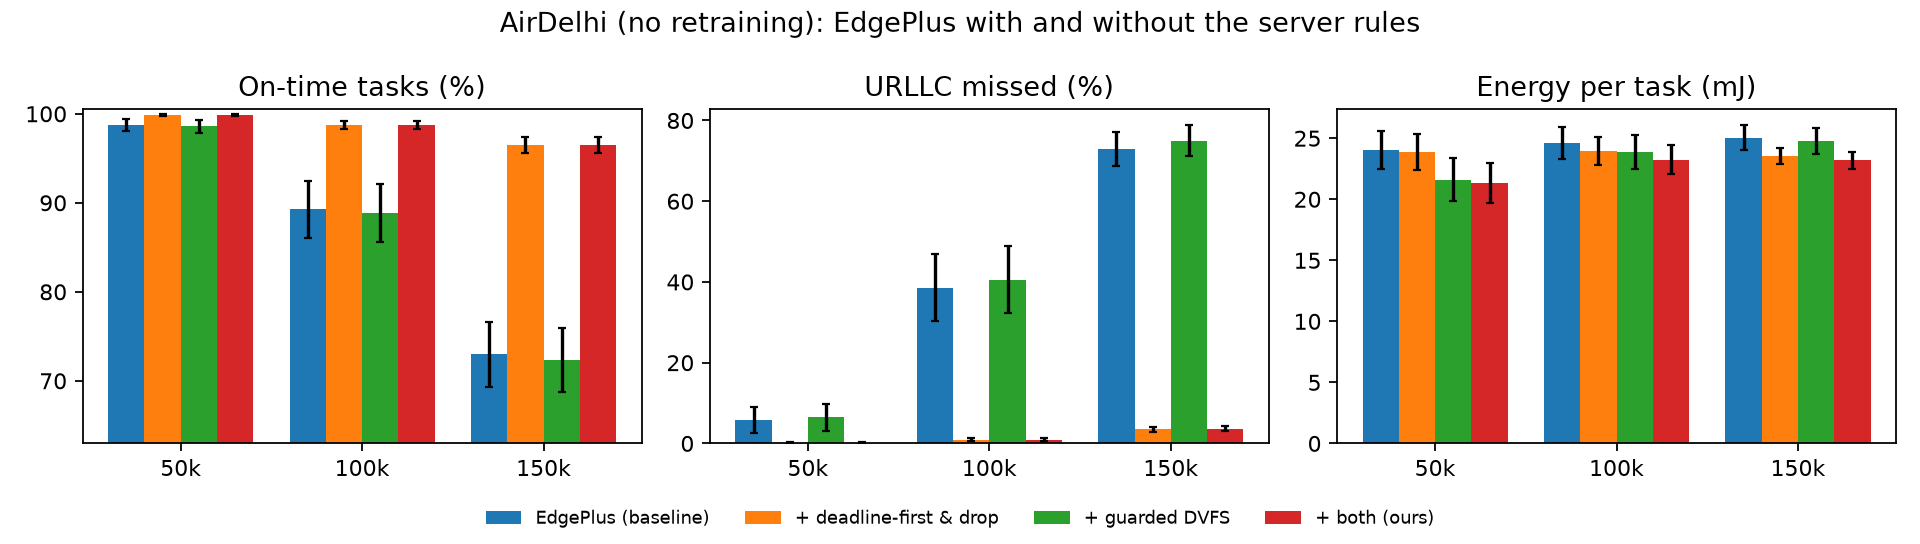
\includegraphics[width=\textwidth]{figures/main_delhi.png}
\caption{AirDelhi (models trained on CityPulse): share of tasks on time, missed URLLC tasks and energy per task.
Error bars are 95\% confidence intervals.}
\label{fig:main_dl}
\end{figure}

\subsection{Which part of the method does what?}
\label{sec:ablation}
To see why the method works, we switched its parts on and off one at a time at the heaviest CityPulse load
(Table~\ref{tab:ablation}, Figure~\ref{fig:ablation}).

\begin{itemize}
\item \textbf{Dropping alone} (still FCFS) raises the on-time share to 91.2\%, but 40.3\% of URLLC tasks still miss
and 8.8\% of all tasks are dropped. Without deadline order, urgent tasks reach the front of the queue too late
and are then dropped.
\item \textbf{Deadline order alone} (no dropping) reaches 97.4\%. In the full city we did not see the dramatic
domino effect of worked example~1, probably because EdgePlus's mask already steers new tasks away from servers
with long queues. Still, without dropping, 4.2\% of eMBB and 1.4\% of mMTC tasks miss.
\item \textbf{Fixed class priority} (URLLC first, then eMBB, then mMTC, with dropping) protects URLLC tasks
(0.11\% missed) but leaves 10.1\% of mMTC tasks late: a relaxed task never gets ahead of an urgent one, even when
its own deadline is about to pass. Deadlines make a better priority than fixed classes.
\item \textbf{Deadline order with dropping} (Rule~1) gives the best on-time share, 99.6\%.
\item \textbf{Unguarded slow-down} is a disaster: only 46.0\% on time at heavy load (and 66.0\% at medium load),
because slowed tasks block cores that urgent tasks need. It saves the most energy at light load (28.1\%), but at
too high a price.
\item \textbf{Guarded slow-down} (Rule~2) keeps the on-time share within one point of EdgePlus at every load, on
both datasets, while saving energy.
\end{itemize}

\begin{table}[!htbp]
\caption{Switching the parts of the method on and off (CityPulse, 150{,}000 tasks, average of 30 runs).}
\label{tab:ablation}
\footnotesize
\begin{tabular*}{\textwidth}{@{\extracolsep\fill}lrrrrrr@{}}
\toprule
 & On time & \multicolumn{3}{c}{Missed (\%)} & 95th pct & Energy\\
\cmidrule(lr){3-5}
Rules & (\%) & URLLC & eMBB & mMTC & latency (s) & (mJ/task)\\
\midrule
EdgePlus (FCFS, keep late tasks) & 80.52 & 55.36 & 16.80 & 0.03 & 148.1 & 28.36\\
Drop late tasks only & 91.24 & 40.33 & 1.39 & 0.00 & 86.7 & 26.46\\
Deadline first only & 97.41 & 0.32 & 4.24 & 1.37 & 298.0 & 28.29\\
Fixed class priority + drop & 96.49 & 0.11 & 0.89 & 10.14 & 171.0 & 27.35\\
Rule 1: deadline first + drop & 99.64 & 0.07 & 0.65 & 0.05 & 290.6 & 28.07\\
Unguarded slow-down & 45.96 & 80.11 & 67.55 & 14.16 & 637.0 & 24.48\\
Rule 2: guarded slow-down & 79.60 & 57.11 & 17.94 & 0.04 & 155.1 & 27.11\\
Both rules (ours) & \textbf{99.65} & 0.07 & 0.64 & 0.05 & 298.4 & 26.88\\
\botrule
\end{tabular*}
\end{table}

\begin{figure}[!htbp]
\centering
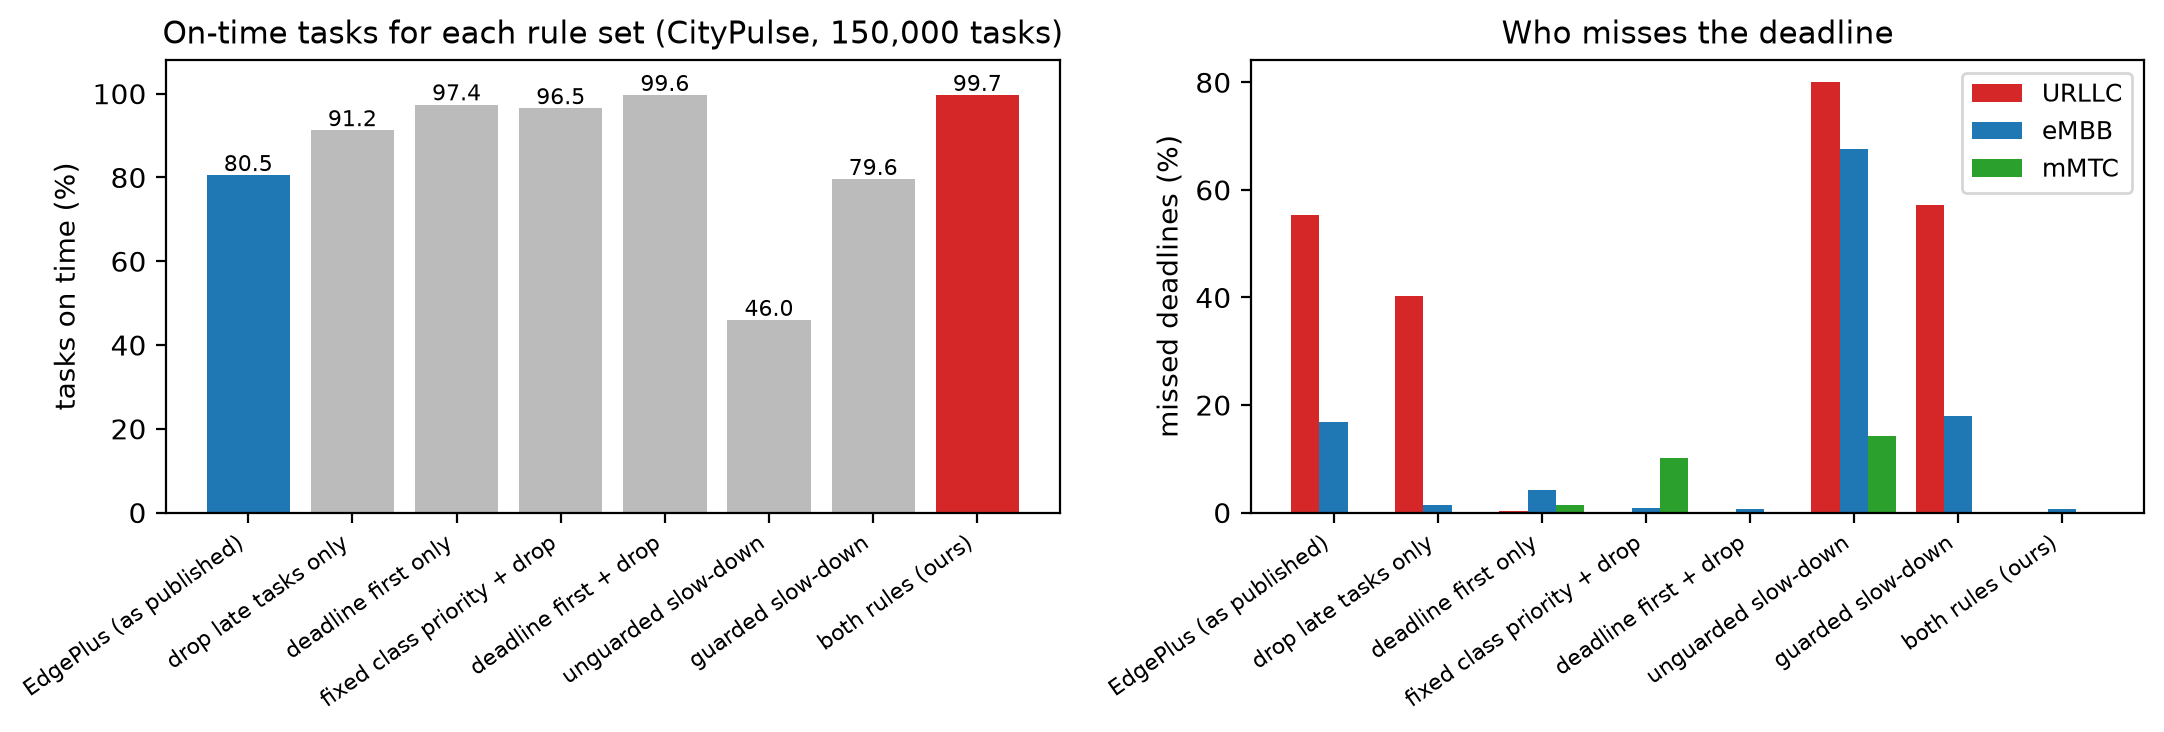
\includegraphics[width=\textwidth]{figures/ablation.png}
\caption{The parts of the method, CityPulse at 150{,}000 tasks. Left: share of tasks on time. Right: missed
deadlines per class.}
\label{fig:ablation}
\end{figure}

\subsection{What happens during an episode}
Figure~\ref{fig:overtime} follows one heavy-load test episode over its 10 minutes and shows the on-time share of
tasks grouped by when they arrived. On CityPulse, EdgePlus starts well, but its queues grow steadily in the busy
clusters, and by the end of the window only about 60\% of new tasks finish on time. With our rules the share stays
near 99\% throughout. On AirDelhi, EdgePlus collapses during each burst, down to about 9\% at the worst moment,
and recovers in between. With our rules the bursts still hurt, but the on-time share stays above 83\% at all
times. In this particular episode the totals are 60.7\% for EdgePlus and 93.9\% for our rules.

\begin{figure}[!htbp]
\centering
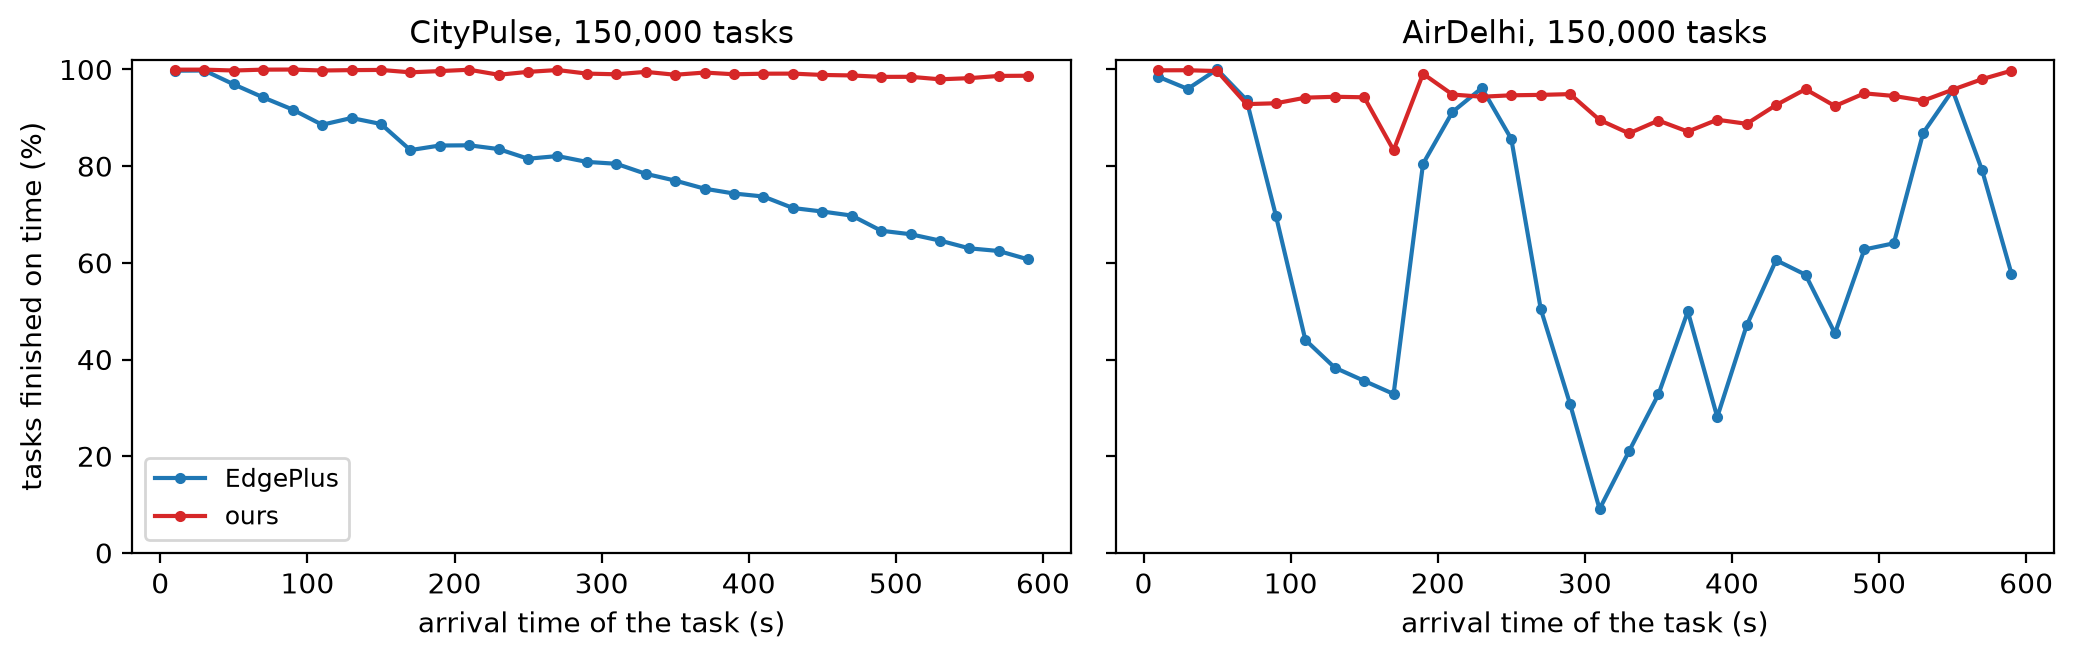
\includegraphics[width=\textwidth]{figures/over_time.png}
\caption{On-time share of tasks by arrival time (20-second groups) in one heavy-load test episode.}
\label{fig:overtime}
\end{figure}

\subsection{Which parts of the city benefit}
Figure~\ref{fig:cluster} breaks the same episodes down by cluster. Quiet clusters were already fine. The gains are
in the busy clusters. On CityPulse, cluster~4, which receives 20\% of all tasks, goes from 60.0\% to 98.0\% on time,
and cluster~8 from 66.4\% to 99.2\%. On AirDelhi the busiest clusters 0, 2 and 6 go from about 45\% to 88--94\%.
The city as a whole also becomes fairer: no area is left far behind.

\begin{figure}[!htbp]
\centering
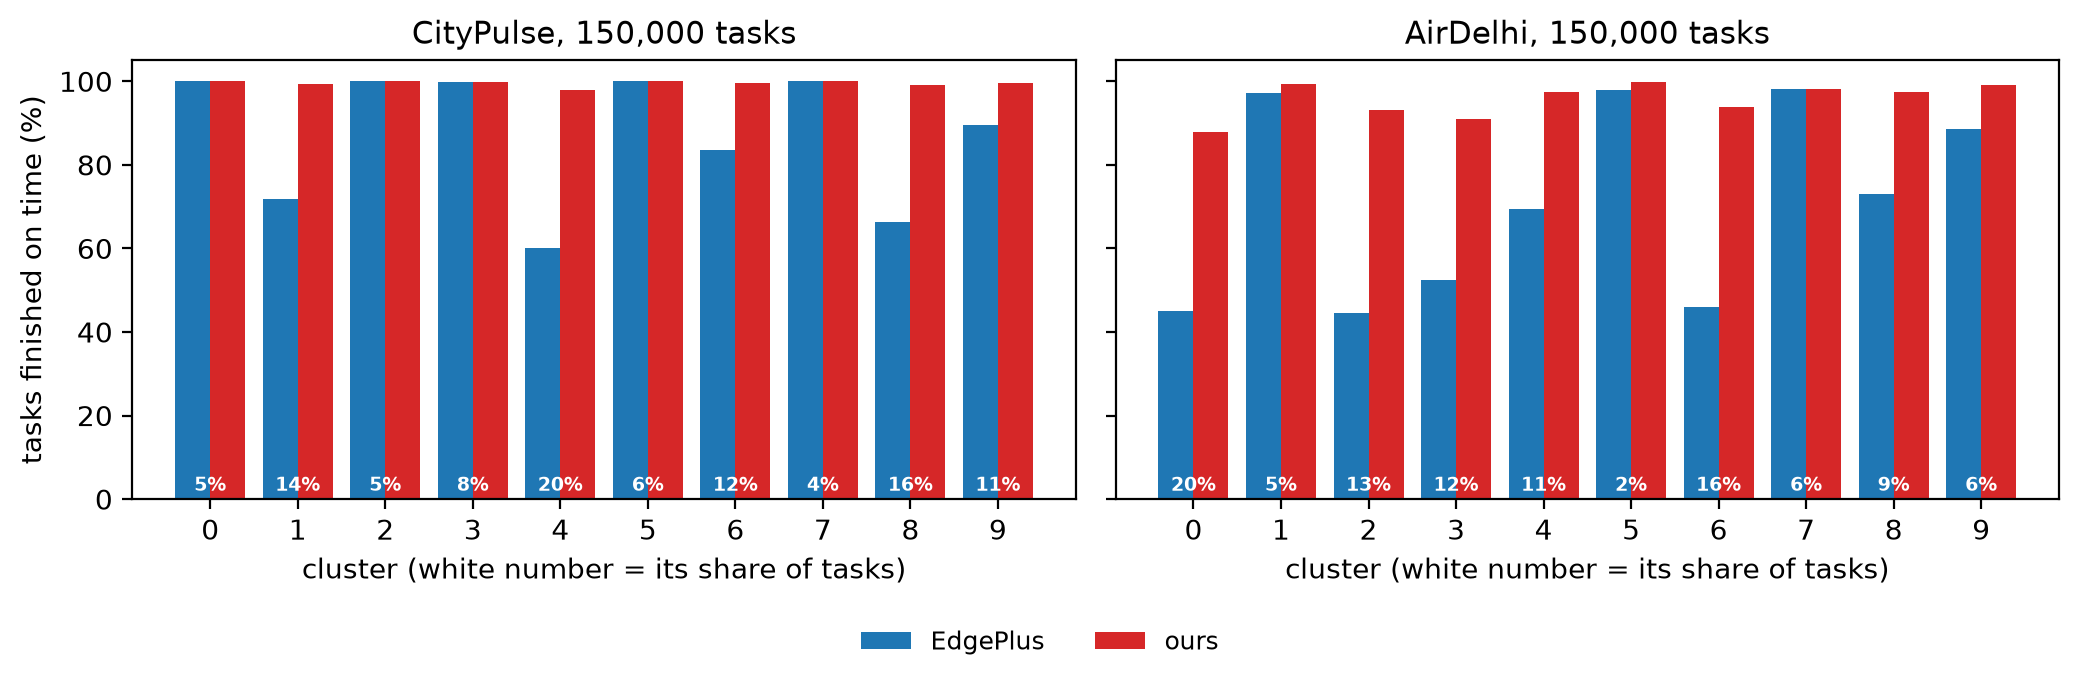
\includegraphics[width=\textwidth]{figures/per_cluster.png}
\caption{On-time share per cluster in one heavy-load test episode. The white number on each bar is the cluster's
share of all tasks.}
\label{fig:cluster}
\end{figure}

\subsection{The price: relaxed tasks wait longer}
Our rules are not free. Deadline order moves waiting time from urgent tasks to relaxed ones
(Figure~\ref{fig:latclass}). On CityPulse at heavy load, the 95th-percentile latency of URLLC tasks falls from 92\,s
to 6\,s and that of eMBB tasks from 105\,s to 87\,s, but that of mMTC tasks rises from 223\,s to 439\,s. Because
mMTC tasks are 30\% of all tasks, the 95th-percentile latency of all tasks together rises from 148\,s to 298\,s.
These relaxed tasks still meet their deadlines of 120--600\,s: only 0.05\% of them miss.

Figure~\ref{fig:cdf} shows the full picture for each class. With our rules almost every URLLC task is done within
its 5--15\,s window, and far more eMBB tasks finish early, while mMTC tasks are deliberately pushed later, though
still inside their window. On AirDelhi the overall 95th-percentile latency at heavy load does not change
significantly (339\,s against 316\,s), and at medium load it rises from 110\,s to 155\,s.

The lesson is that a single latency number over all classes can be misleading when deadlines range from 5 to
600 seconds. A system that finishes a logging task in 400 seconds instead of 200 has lost nothing if the deadline
is 600 seconds. Latency is best reported per class, next to the share of deadlines met.

\begin{figure}[!htbp]
\centering
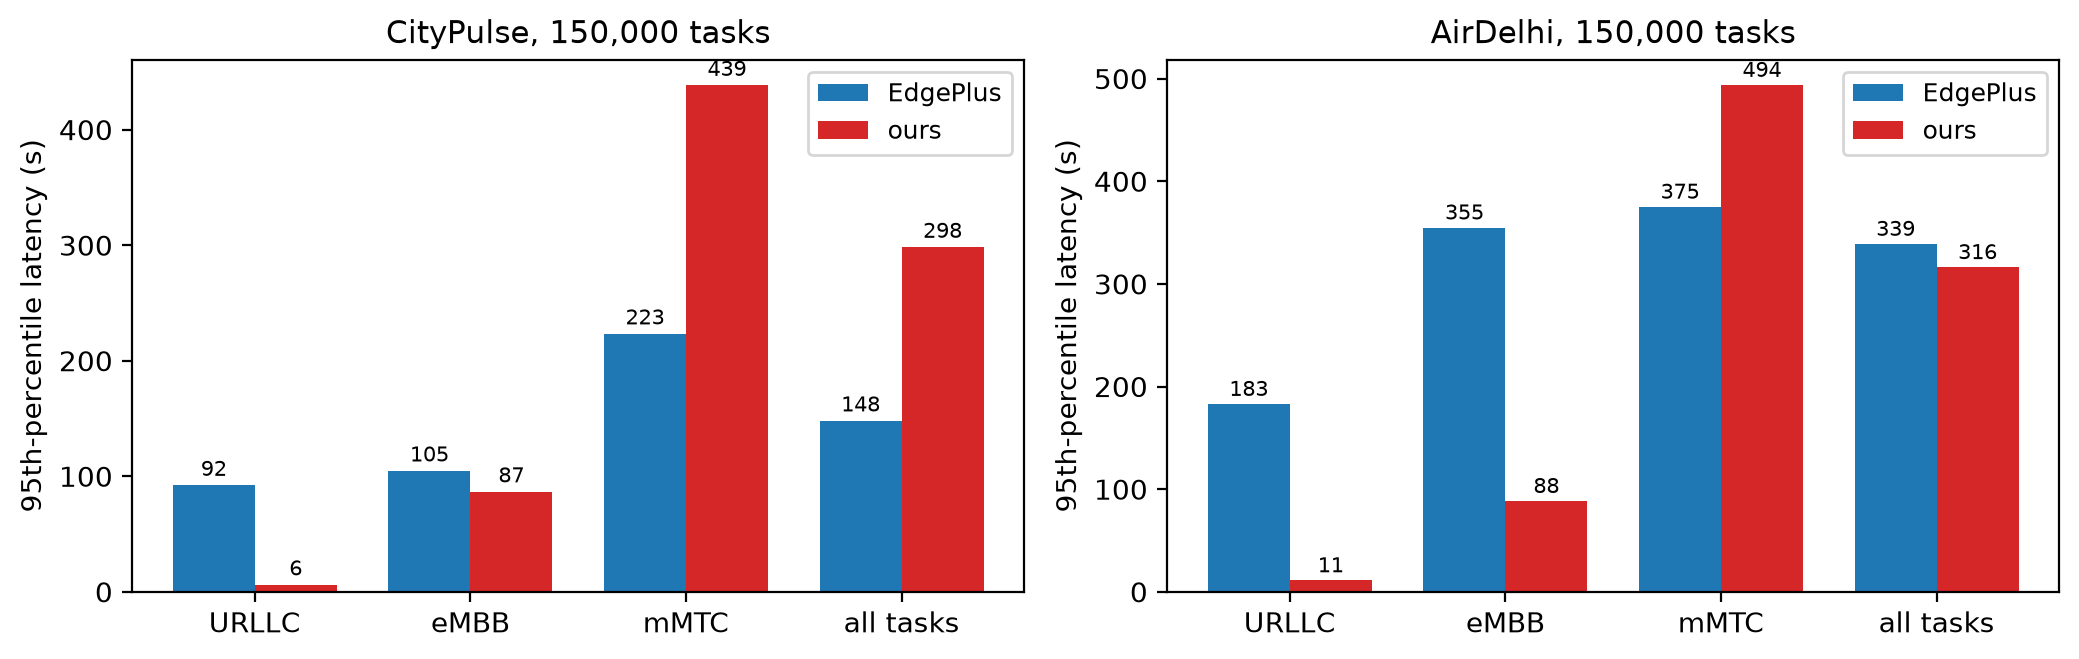
\includegraphics[width=\textwidth]{figures/latency_by_class.png}
\caption{95th-percentile latency by class at heavy load (average of 30 runs).}
\label{fig:latclass}
\end{figure}

\begin{figure}[!htbp]
\centering
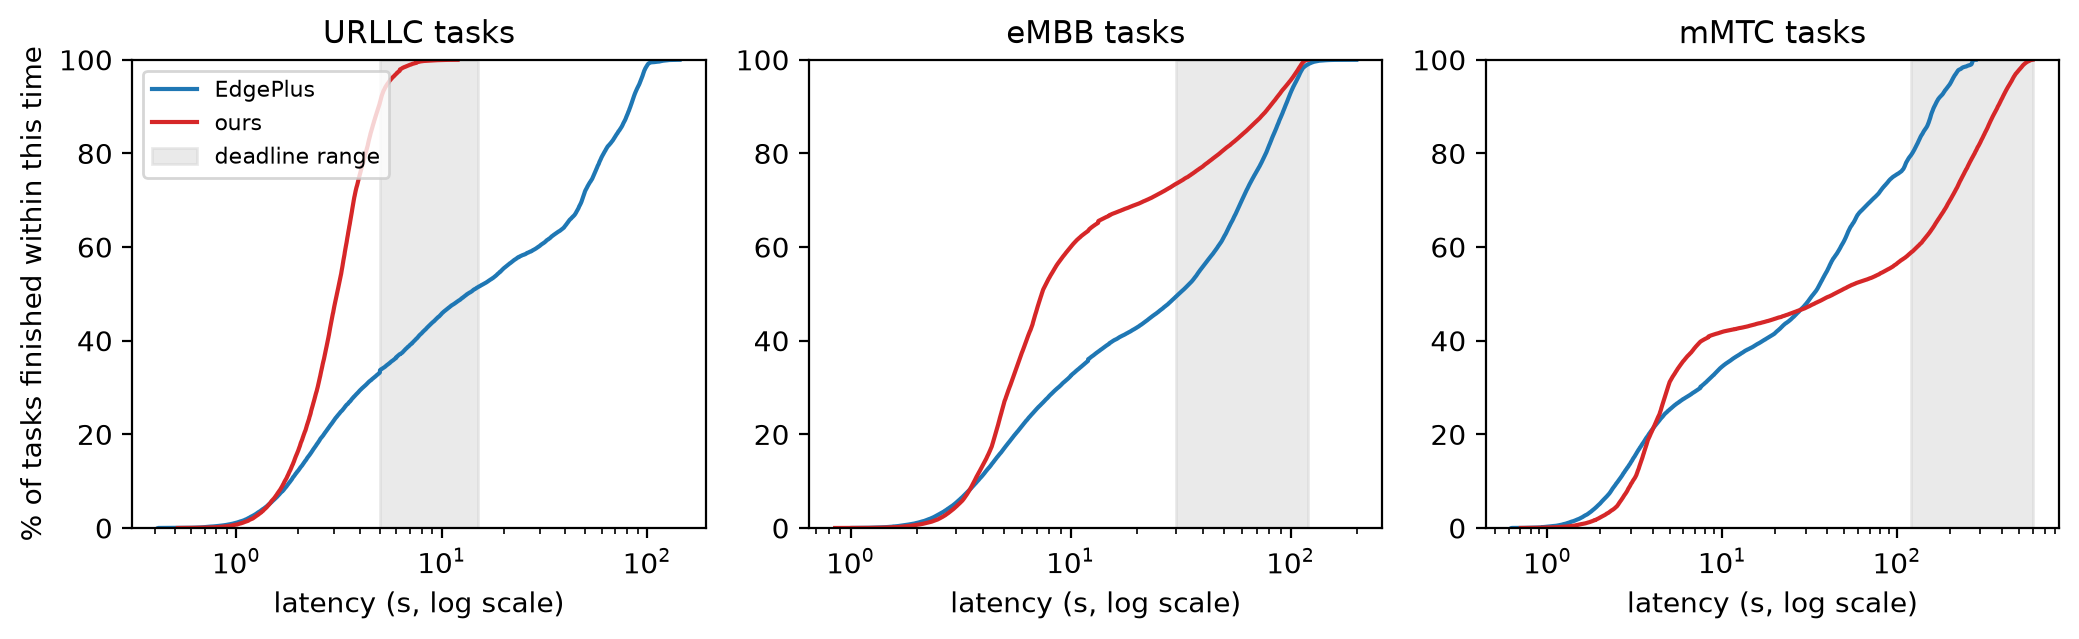
\includegraphics[width=\textwidth]{figures/latency_cdf.png}
\caption{How quickly tasks of each class finish (CityPulse, one heavy-load test episode). A curve that rises
further to the left means faster. The grey band is the class's deadline range.}
\label{fig:cdf}
\end{figure}

\subsection{Energy savings in detail}
Figure~\ref{fig:energy} shows how the energy saving depends on load. The saving comes almost entirely from Rule~2
on CityPulse (dashed and solid blue lines overlap). Rule~2 slows down 97.8\% of tasks at light load but only 21.9\%
at heavy load, because a busy server rarely has an empty queue. On AirDelhi the combination saves more than
Rule~2 alone at medium and heavy load (5.5\% against 2.9\%, and 7.3\% against 1.1\%): Rule~1 also saves energy,
because it does not spend CPU time on tasks that are already lost.

Figure~\ref{fig:speeds} shows which speeds the rule actually picks. At light load most tasks run at 70--80\% of
full speed, and almost none at full speed. At heavy load, 74\% of tasks still run at full speed. The rule
naturally backs off when the city is busy.

\begin{figure}[!htbp]
\centering
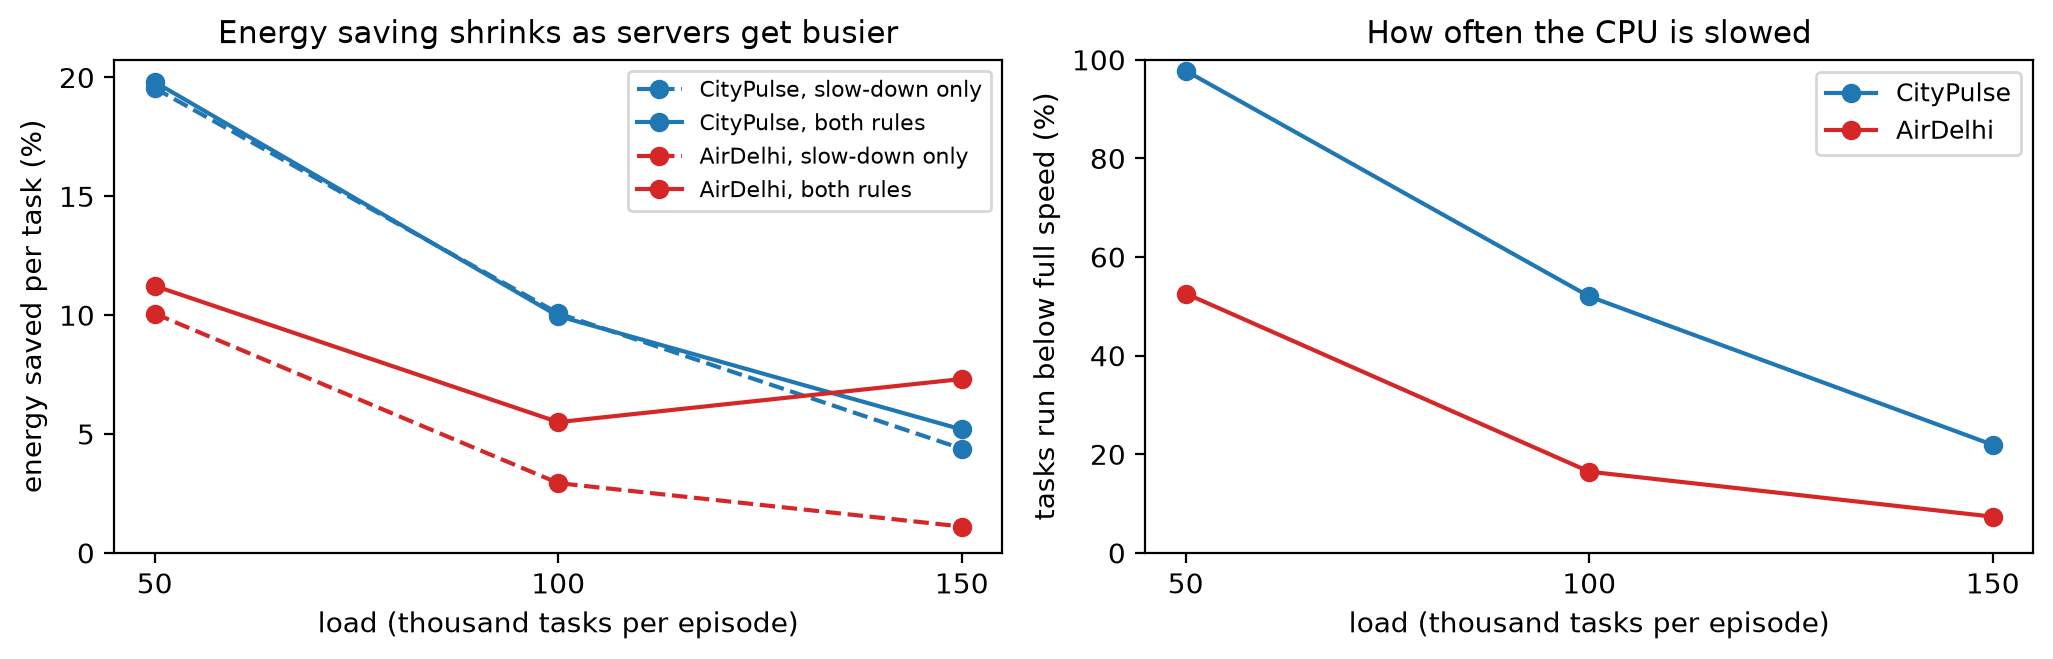
\includegraphics[width=\textwidth]{figures/energy_savings.png}
\caption{Left: energy saved per task compared with EdgePlus. Right: share of tasks run below full speed.}
\label{fig:energy}
\end{figure}

\begin{figure}[!htbp]
\centering
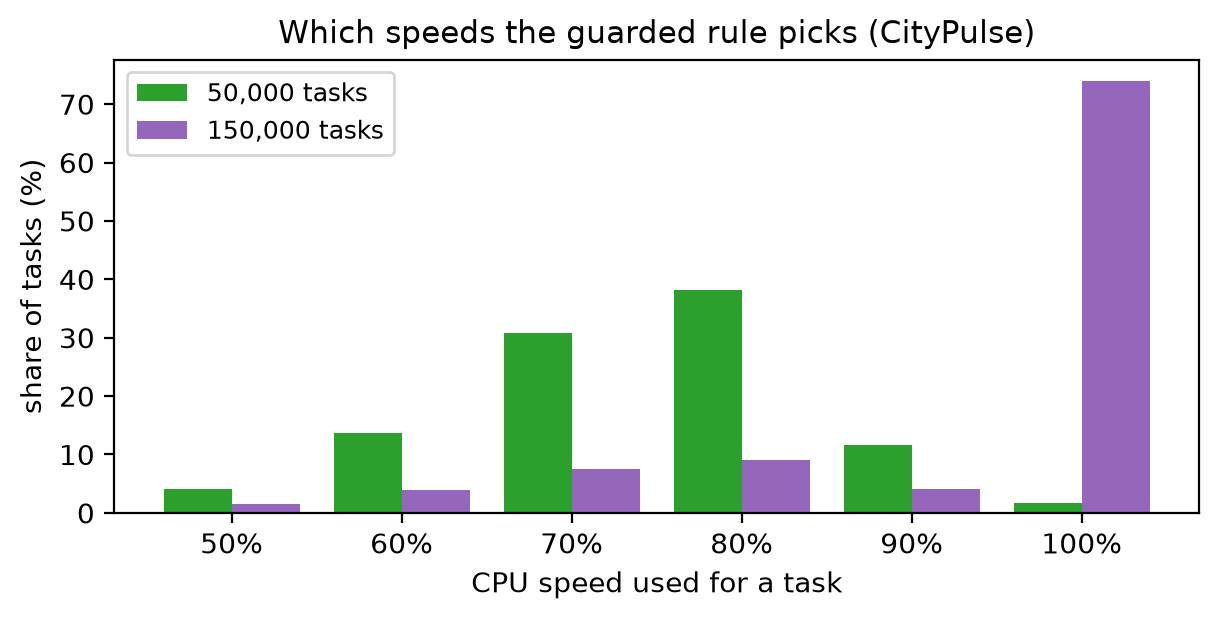
\includegraphics[width=0.68\textwidth]{figures/speeds.png}
\caption{CPU speeds chosen by the guarded rule in one CityPulse test episode at light and heavy load.}
\label{fig:speeds}
\end{figure}

\subsection{Are the differences real?}
Table~\ref{tab:stats} gives the paired statistical tests for our full method against EdgePlus. Every difference
in on-time share and energy is statistically significant. The tests are worth reading carefully at light
CityPulse load: there our rules lower the on-time share by 0.002 points, about two tasks in 100{,}000. The test
correctly says this difference is real, but it is far too small to matter in practice.

\begin{table}[!htbp]
\caption{Paired tests of our full method against EdgePlus (30 pairs each, Wilcoxon signed-rank test,
Benjamini--Hochberg adjusted p-values). A p-value below 0.05 means the difference is very unlikely to be luck.}
\label{tab:stats}
\small
\begin{tabular*}{\textwidth}{@{\extracolsep\fill}llrlrlrl@{}}
\toprule
Data & Load & \multicolumn{2}{c}{On time} & \multicolumn{2}{c}{Energy per task} & \multicolumn{2}{c}{95th-pct latency}\\
\cmidrule(lr){3-4}\cmidrule(lr){5-6}\cmidrule(lr){7-8}
 & & change & p & change & p & change & p\\
\midrule
CityPulse & 50{,}000 & $-$0.002 pts & 0.0005 & $-$19.8\% & $<$0.0001 & +0.8\,s & $<$0.0001\\
 & 100{,}000 & +0.12 pts & $<$0.0001 & $-$10.0\% & $<$0.0001 & $-$1.3\,s & $<$0.0001\\
 & 150{,}000 & +19.13 pts & $<$0.0001 & $-$5.2\% & $<$0.0001 & +150.3\,s & $<$0.0001\\
AirDelhi & 50{,}000 & +1.09 pts & $<$0.0001 & $-$11.2\% & $<$0.0001 & +3.1\,s & $<$0.0001\\
 & 100{,}000 & +9.51 pts & $<$0.0001 & $-$5.5\% & $<$0.0001 & +45.4\,s & $<$0.0001\\
 & 150{,}000 & +23.50 pts & $<$0.0001 & $-$7.3\% & $<$0.0001 & $-$22.7\,s & 0.74\\
\botrule
\end{tabular*}
\end{table}

\subsection{Do the rules need a learned scheduler?}
Finally, we applied the same rules to the simple, non-learning scheduler from Section~\ref{sec:setup}, which sends
each task to the first server in routing order that can finish it in time. On CityPulse at heavy load the rules
raise it from 72.0\% to 98.8\% on time, and at light load they cut its energy per task by 10.7\%. So the rules
help on their own, but the best results come from combining them with the learned EdgePlus policy (99.7\% on
time). The learned policy and the server rules solve different parts of the problem: one picks the right server,
the other uses that server well.

%=====================================================================================================
\section{Discussion}
\label{sec:discussion}
%=====================================================================================================

\subsection{What this means in practice}
\begin{enumerate}
\item \textbf{Choosing a good server is not enough.} Even a strong learned scheduler loses many urgent tasks if
servers then work through their queues in arrival order. The order inside the server matters as much as the
choice of server.
\item \textbf{Use deadlines as priorities, and drop lost causes.} Deadline order protects urgent tasks without
starving relaxed ones, and dropping hopeless tasks frees time for tasks that can still be saved.
\item \textbf{Save energy only when it is safe.} Slowing the CPU is a cheap way to save energy, but only when no
other work is waiting, and only by a bounded amount.
\item \textbf{Report results per class.} Overall numbers hid the fact that all of EdgePlus's misses were urgent and
routine tasks (57\% and 43\% of the misses at heavy load), while relaxed tasks almost never missed.
\end{enumerate}

\subsection{Limitations}
We want to be clear about what our results do and do not show.
\begin{itemize}
\item All results come from a simulator. We checked it against the EdgePlus paper, but the size of the gains
depends on choices such as multi-core servers and the deadline ranges.
\item Our EdgePlus rebuild leaves out PSO, the security layer and the original path planner, and uses three
training seeds per load. At medium load it is much less congested than the original on CityPulse.
\item CityPulse values are generated, not measured. AirDelhi is real, but we only tested models trained on
CityPulse there; training directly on Delhi data might change the baseline.
\item Dropping assumes a late result is worthless. If late logging results are still useful, dropping could be
limited to URLLC and eMBB tasks.
\item Our energy model uses a 25\% static share and speeds down to half; it does not include idle power or sleep
modes, which could save more at light load.
\item Relaxed tasks wait longer. Applications that care about absolute delay rather than deadlines may not want
this trade-off.
\end{itemize}

\subsection{Future work}
Natural next steps are to retrain EdgePlus with the rules switched on, so that it learns to make use of them; to
train and test on real data from more cities; to add idle power and sleep modes to the energy model; and to
bring back the PSO outer loop for a complete comparison with the original system.

%=====================================================================================================
\section{Conclusion}
%=====================================================================================================

EdgePlus decides which server should run each task in a 6G edge network, but treats all tasks the same once they
reach a server. We added two simple rules inside each server: run the task with the earliest deadline first and
drop tasks that can no longer make it, and slow the CPU down only when nothing else is waiting and only by a
bounded amount. With the same trained EdgePlus model, these rules raise the share of tasks finished on time at
heavy load from 80.5\% to 99.7\% on the CityPulse data and from 73.0\% to 96.5\% on real data from Delhi, and cut
energy per task by up to 19.8\% at light load. The price is a longer, but still on-time, wait for relaxed tasks.
The experiments also show why each detail matters: deadline order works best together with dropping, deadlines
make better priorities than fixed classes, and slowing down the CPU needs a guard.

\backmatter

\bmhead{Code and data availability}

The simulator, the trained models, all raw results and the scripts that produce every table and figure in this
paper are available in the project repository. CityPulse and AirDelhi are public datasets; AirDelhi is released
under the CC BY 4.0 licence.

%% Springer Nature journals usually require a Declarations section, for example:
%% \section*{Declarations}
%% \begin{itemize}
%% \item Funding
%% \item Conflict of interest/Competing interests
%% \item Ethics approval and consent to participate
%% \item Consent for publication
%% \item Data availability
%% \item Materials availability
%% \item Code availability
%% \item Author contribution
%% \end{itemize}

\begin{appendices}

\section{All simulation parameters}
\label{app:params}

\begin{table}[!htbp]
\caption{Parameters of the simulator and of training. Values marked $^\dagger$ come from the EdgePlus paper.}
\small
\begin{tabularx}{\textwidth}{lL}
\toprule
Parameter & Value\\
\midrule
City & 10\,km $\times$ 10\,km$^\dagger$, 10 clusters$^\dagger$, weighted K-means and Delaunay neighbours$^\dagger$\\
Task classes & URLLC / eMBB / mMTC = 20 / 50 / 30\%$^\dagger$; deadlines 5--15, 30--120, 120--600\,s$^\dagger$\\
CPU work per task & averages 6 / 12 / 9 Gcycles; spread $\sigma=0.47$ (log-normal); about 16\% more per unit of severity\\
Data per task & 2 / 8 / 1\,KB; memory 64 / 128 / 32\,MB\\
Loads & 50{,}000 / 100{,}000 / 150{,}000 tasks in a 600\,s window$^\dagger$\\
Radio & 20 / 50 / 5\,MHz per class; frequency reuse 3; 23\,dBm power + 20\,dB antenna gain; path loss
$128.1 + 37.6\log_{10} d$ (d in km) \cite{3gpp36814}; MAC efficiency 0.7; overhead 1.2\\
Slices & 25 / 65 / 35\% of a cluster's cores reserved per class over a 60\,s window\\
Energy & 2.2 / 2.8 / 1.8\,mJ per Gcycle (stationary / mobile / cloud) at full speed; 25\% static; device radio 0.2\,W;
4\,mJ per task sent to the cloud; 0.02\,mJ per metre driven\\
Rule 2 & speeds 50--100\% in steps of 10\%; at most 80\% of the slack and 1.5\,s extra\\
Ledger signals & reputation: moving average of on-time results (weight 0.05); threshold 0.6$^\dagger$; URLLC avoids
servers below 0.4; debt target 0.9\\
Advisory & bonus weights: Nash 0.5, PID 0.5, leader 0.3; PID gains 1.90 / 1.20 / 0.06$^\dagger$; set point 80\%;
mobile servers move every 20\,s\\
Reward & weights 1, 1, 0.2, 0.1, 0.2, 0.5, 0.5 for on time, late, latency, energy, cloud, reputation, debt; class
weights 3 / 1.5 / 1\\
PPO & 60 rounds; discount 0.95; GAE 0.9 \cite{schulman2016gae}; clip 0.2; 4 passes per round; batches of 4096;
learning rate 0.0003; entropy bonus 0.01\\
Networks & actor: 2 layers of 64 units; critic: 2 layers of 128 units; up to 16 candidate servers per decision\\
Tests & 3 training seeds $\times$ 10 test episodes per load; models run greedily (always the best-scored server)\\
\botrule
\end{tabularx}
\end{table}

\end{appendices}

\bibliography{refs}% references are formatted by sn-mathphys-num.bst

\end{document}
